\documentclass[10pt,a4paper]{book}
\usepackage{lmodern}
\usepackage{amssymb,amsmath}
\usepackage{ifxetex,ifluatex}
\usepackage{fixltx2e} % provides \textsubscript
\ifnum 0\ifxetex 1\fi\ifluatex 1\fi=0 % if pdftex
  \usepackage[T1]{fontenc}
  \usepackage[utf8]{inputenc}
\else % if luatex or xelatex
  \ifxetex
    \usepackage{mathspec}
  \else
    \usepackage{fontspec}
  \fi
  \defaultfontfeatures{Ligatures=TeX,Scale=MatchLowercase}
\fi
% use upquote if available, for straight quotes in verbatim environments
\IfFileExists{upquote.sty}{\usepackage{upquote}}{}
% use microtype if available
\IfFileExists{microtype.sty}{%
\usepackage[]{microtype}
\UseMicrotypeSet[protrusion]{basicmath} % disable protrusion for tt fonts
}{}
\PassOptionsToPackage{hyphens}{url} % url is loaded by hyperref
\usepackage[unicode=true]{hyperref}
\PassOptionsToPackage{usenames,dvipsnames}{color} % color is loaded by hyperref
\hypersetup{
            pdftitle={Estatística Computacional com R},
            pdfauthor={Fernando P. Mayer; Wagner H. Bonat},
            colorlinks=true,
            linkcolor=Maroon,
            citecolor=Blue,
            urlcolor=Blue,
            breaklinks=true}
\urlstyle{same}  % don't use monospace font for urls
\usepackage[margin=3cm]{geometry}
\usepackage{color}
\usepackage{fancyvrb}
\newcommand{\VerbBar}{|}
\newcommand{\VERB}{\Verb[commandchars=\\\{\}]}
\DefineVerbatimEnvironment{Highlighting}{Verbatim}{commandchars=\\\{\}}
% Add ',fontsize=\small' for more characters per line
\usepackage{framed}
\definecolor{shadecolor}{RGB}{248,248,248}
\newenvironment{Shaded}{\begin{snugshade}}{\end{snugshade}}
\newcommand{\KeywordTok}[1]{\textcolor[rgb]{0.13,0.29,0.53}{\textbf{#1}}}
\newcommand{\DataTypeTok}[1]{\textcolor[rgb]{0.13,0.29,0.53}{#1}}
\newcommand{\DecValTok}[1]{\textcolor[rgb]{0.00,0.00,0.81}{#1}}
\newcommand{\BaseNTok}[1]{\textcolor[rgb]{0.00,0.00,0.81}{#1}}
\newcommand{\FloatTok}[1]{\textcolor[rgb]{0.00,0.00,0.81}{#1}}
\newcommand{\ConstantTok}[1]{\textcolor[rgb]{0.00,0.00,0.00}{#1}}
\newcommand{\CharTok}[1]{\textcolor[rgb]{0.31,0.60,0.02}{#1}}
\newcommand{\SpecialCharTok}[1]{\textcolor[rgb]{0.00,0.00,0.00}{#1}}
\newcommand{\StringTok}[1]{\textcolor[rgb]{0.31,0.60,0.02}{#1}}
\newcommand{\VerbatimStringTok}[1]{\textcolor[rgb]{0.31,0.60,0.02}{#1}}
\newcommand{\SpecialStringTok}[1]{\textcolor[rgb]{0.31,0.60,0.02}{#1}}
\newcommand{\ImportTok}[1]{#1}
\newcommand{\CommentTok}[1]{\textcolor[rgb]{0.56,0.35,0.01}{\textit{#1}}}
\newcommand{\DocumentationTok}[1]{\textcolor[rgb]{0.56,0.35,0.01}{\textbf{\textit{#1}}}}
\newcommand{\AnnotationTok}[1]{\textcolor[rgb]{0.56,0.35,0.01}{\textbf{\textit{#1}}}}
\newcommand{\CommentVarTok}[1]{\textcolor[rgb]{0.56,0.35,0.01}{\textbf{\textit{#1}}}}
\newcommand{\OtherTok}[1]{\textcolor[rgb]{0.56,0.35,0.01}{#1}}
\newcommand{\FunctionTok}[1]{\textcolor[rgb]{0.00,0.00,0.00}{#1}}
\newcommand{\VariableTok}[1]{\textcolor[rgb]{0.00,0.00,0.00}{#1}}
\newcommand{\ControlFlowTok}[1]{\textcolor[rgb]{0.13,0.29,0.53}{\textbf{#1}}}
\newcommand{\OperatorTok}[1]{\textcolor[rgb]{0.81,0.36,0.00}{\textbf{#1}}}
\newcommand{\BuiltInTok}[1]{#1}
\newcommand{\ExtensionTok}[1]{#1}
\newcommand{\PreprocessorTok}[1]{\textcolor[rgb]{0.56,0.35,0.01}{\textit{#1}}}
\newcommand{\AttributeTok}[1]{\textcolor[rgb]{0.77,0.63,0.00}{#1}}
\newcommand{\RegionMarkerTok}[1]{#1}
\newcommand{\InformationTok}[1]{\textcolor[rgb]{0.56,0.35,0.01}{\textbf{\textit{#1}}}}
\newcommand{\WarningTok}[1]{\textcolor[rgb]{0.56,0.35,0.01}{\textbf{\textit{#1}}}}
\newcommand{\AlertTok}[1]{\textcolor[rgb]{0.94,0.16,0.16}{#1}}
\newcommand{\ErrorTok}[1]{\textcolor[rgb]{0.64,0.00,0.00}{\textbf{#1}}}
\newcommand{\NormalTok}[1]{#1}
\usepackage{longtable,booktabs}
% Fix footnotes in tables (requires footnote package)
\IfFileExists{footnote.sty}{\usepackage{footnote}\makesavenoteenv{long table}}{}
\IfFileExists{parskip.sty}{%
\usepackage{parskip}
}{% else
\setlength{\parindent}{0pt}
\setlength{\parskip}{6pt plus 2pt minus 1pt}
}
\setlength{\emergencystretch}{3em}  % prevent overfull lines
\providecommand{\tightlist}{%
  \setlength{\itemsep}{0pt}\setlength{\parskip}{0pt}}
\setcounter{secnumdepth}{5}
% Redefines (sub)paragraphs to behave more like sections
\ifx\paragraph\undefined\else
\let\oldparagraph\paragraph
\renewcommand{\paragraph}[1]{\oldparagraph{#1}\mbox{}}
\fi
\ifx\subparagraph\undefined\else
\let\oldsubparagraph\subparagraph
\renewcommand{\subparagraph}[1]{\oldsubparagraph{#1}\mbox{}}
\fi

% set default figure placement to htbp
\makeatletter
\def\fps@figure{htbp}
\makeatother

%%----------------------------------------------------------------------
%% Opções comuns
\usepackage[brazil]{babel}
\usepackage[T1]{fontenc}
\usepackage{amsmath,amsfonts,amssymb,amsthm}
%%----------------------------------------------------------------------

%%----------------------------------------------------------------------
%% FLOATS: graficos e tabelas
\usepackage{graphicx}
%%----------------------------------------------------------------------

%%----------------------------------------------------------------------
%% hyperref e xcolor
\usepackage{hyperref} % hidelinks
\usepackage{xcolor}
\hypersetup{
    colorlinks,
    linkcolor={red!50!black},
    citecolor={blue!50!black},
    urlcolor={blue!80!black}
}
%%----------------------------------------------------------------------

%%----------------------------------------------------------------------
%% FONTES
%% micro-tipografia
% \usepackage[protrusion=true,expansion=true]{microtype}
%% Bitstream Charter with mathdesign
%\usepackage{lmodern} % sans-serif: Latin Modern
% \usepackage[charter]{mathdesign} % serif: Bitstream Charter
%\usepackage[scaled]{beramono} % truetype: Bistream Vera Sans Mono
% \usepackage[scaled]{helvet}
\usepackage{mathpazo}
\usepackage{inconsolata}
%%----------------------------------------------------------------------

\title{Estatística Computacional com R}
\author{Fernando P. Mayer \and Wagner H. Bonat}
\date{Laboratório de Estatística e Geoinformação (LEG)\\
Departamento de Estatística (DEST)\\
Universidade Federal do Paraná (UFPR)\\[2\baselineskip]2018-07-24\\
Última atualização: 2018-07-25}

\begin{document}
\maketitle

{
\hypersetup{linkcolor=black}
\setcounter{tocdepth}{2}
\tableofcontents
}
\chapter*{Prefácio}\label{prefacio}


Alguma coisa aqui.

\section{Informação de Sessão}\label{informacao-de-sessao}

\begin{verbatim}
Wednesday, 25 July, 2018, 00:24
----------------------------------------
R version 3.5.0 (2017-01-27)
Platform: x86_64-pc-linux-gnu (64-bit)
Running under: Ubuntu 14.04.5 LTS

Matrix products: default
BLAS: /home/travis/R-bin/lib/R/lib/libRblas.so
LAPACK: /home/travis/R-bin/lib/R/lib/libRlapack.so

locale:
 [1] LC_CTYPE=en_US.UTF-8       LC_NUMERIC=C              
 [3] LC_TIME=en_US.UTF-8        LC_COLLATE=en_US.UTF-8    
 [5] LC_MONETARY=en_US.UTF-8    LC_MESSAGES=en_US.UTF-8   
 [7] LC_PAPER=en_US.UTF-8       LC_NAME=C                 
 [9] LC_ADDRESS=C               LC_TELEPHONE=C            
[11] LC_MEASUREMENT=en_US.UTF-8 LC_IDENTIFICATION=C       

attached base packages:
[1] stats     graphics  grDevices utils     datasets  methods   base     

other attached packages:
[1] knitr_1.20

loaded via a namespace (and not attached):
 [1] Rcpp_0.12.18    bookdown_0.7.15 digest_0.6.15   rprojroot_1.3-2
 [5] backports_1.1.2 magrittr_1.5    evaluate_0.11   highr_0.7      
 [9] stringi_1.2.4   rstudioapi_0.7  rmarkdown_1.10  tools_3.5.0    
[13] stringr_1.3.1   xfun_0.3        yaml_2.1.19     compiler_3.5.0 
[17] htmltools_0.3.6
\end{verbatim}

\chapter{Computação científica e interação com o
R}\label{computacao-cientifica-e-interacao-com-o-r}

\section{Interagindo com o
computador}\label{interagindo-com-o-computador}

O que significa este ícone?

\begin{center}
\includegraphics[width=0.5\linewidth]{img/excelcsvgrey} \end{center}

\begin{itemize}
\tightlist
\item
  É um documento do Microsoft Excel?
\item
  É um arquivo de \textbf{texto pleno}, separado por vírgulas (CSV
  \emph{comma separated values})
\item
  De fato, o nome do arquivo é \texttt{final.csv} e não \texttt{final}
\item
  O Excel pode sim abrir este arquivo\ldots{} assim como milhares de
  outros programas!
\end{itemize}

O que está acontecendo?

\begin{itemize}
\tightlist
\item
  O computador (leia-se, nesse caso, o sistema operacional Windows)
  ``proteje'' o usuário dos detalhes sujos
\item
  Isso é ruim? \textbf{Sim!}
\item
  O usuário se acostuma com o computador ditando as regras
\item
  É importante lembrar que é você quem deve dizer o que o computador
  deve fazer (nesse caso, com qual programa abrir certo arquivo)
\end{itemize}

O que deve acontecer?

\begin{itemize}
\tightlist
\item
  Para a maioria dos usuários, a interação com o computador se limita a
  clicar em links, selecionar menus e caixas de diálogo
\item
  O problema com essa abordagem é que parece que o usuário é controlado
  pelo computador
\item
  A verdade deve ser o oposto!
\item
  É o usuário que possui o controle e deve dizer para o computador
  exatamente o que fazer
\item
  Escrever código ainda tem a vantagem de deixar registrado tudo o que
  foi feito
\end{itemize}

\section{Editores de texto}\label{editores-de-texto}

Uma característica importante de códigos de programação é que eles são
em \textbf{texto puro}, por isso precisamos de um bom \textbf{editor de
textos}

Características de um bom editor:

\begin{itemize}
\tightlist
\item
  \textbf{Identação automática}
\item
  \textbf{Complementação de parênteses}
\item
  \textbf{Destaque de sintaxe} (\emph{syntax highlighting})
\item
  \textbf{Numeração de linhas}
\item
  \textbf{Auto completar comandos}
\end{itemize}

\subsection{Editores para R}\label{editores-para-r}

Windows:

\begin{itemize}
\tightlist
\item
  Interface padrão: pouco recomendado
\item
  Tinn-R
\end{itemize}

Linux:

\begin{itemize}
\tightlist
\item
  Vim-R-plugin
\item
  Gedit-R-plugin
\end{itemize}

Todas as plataformas:

\begin{itemize}
\tightlist
\item
  Rstudio: recomendado para iniciantes
\item
  Emacs + ESS: altamente recomendado
\end{itemize}

\section{R}\label{r}

\begin{quote}
\emph{``The statistical software should help, by supporting each step
from user to programmer, with as few intrusive barriers as possible.''}
\end{quote}

\begin{quote}
\emph{``\ldots{} to turn ideas into software, quickly and faithfully.''}
\end{quote}

--- John M. Chambers

O R é um dialeto do S e:

\begin{itemize}
\item
  \emph{Ambiente} estatístico para análise de dados e produção de
  gráficos
\item
  Uma completa linguagem de programação:

  \begin{itemize}
  \tightlist
  \item
    Interpretada (contrário de compilada)
  \item
    Orientada a objetos:
  \end{itemize}

  \emph{Tudo no R é um objeto\ldots{}}
\item
  Livre distribuição (código-aberto)
\item
  Mais de 10000 pacotes adicionais
\end{itemize}

Pequeno histórico:

\begin{itemize}
\tightlist
\item
  1980: Linguagem S: desenvolvida por R. Becker, J. Chambers e A. Wilks
  (AT\&T Bell Laboratories)
\item
  1980: Versão comercial: S-Plus (Insightful Corporation)
\item
  1996: Versão livre: R desenvolvido por R. Ihaka e R. Gentleman
  (Universidade de Auckland)
\item
  1997: R Development Core Team
\item
  Hoje: 20 desenvolvedores principais e muitos outros colaboradores em
  todo o mundo
\item
  Estatísticos, matemáticos e programadores
\end{itemize}

\subsection{Configuração inicial}\label{configuracao-inicial}

\begin{itemize}
\item
  O \textbf{diretório de trabalho} é uma pasta onde o R será
  direcionado. Todos os arquivos que serão importados (base de dados,
  \ldots{}) ou exportados (base de dados, gráficos, \ldots{}) por ele
  ficarão nesta pasta.
\item
  Existem duas maneiras de configurar o diretório de trabalho (suponha
  que vamos usar a pasta \texttt{\textasciitilde{}/estatcomp1}):
\item
  \texttt{1)} Utilizando a função \texttt{setwd()} dentro do R:
\end{itemize}

\begin{Shaded}
\begin{Highlighting}[]
\KeywordTok{setwd}\NormalTok{(}\StringTok{"~/estatcomp1"}\NormalTok{)}
\end{Highlighting}
\end{Shaded}

\begin{itemize}
\tightlist
\item
  \texttt{2)} Pelo menu do RStudio em
  \texttt{Session\ \textgreater{}\ Set\ Working\ Directory\ \textgreater{}\ Choose\ Directory...}
  Confira o diretório que está trabalhando com a função
\end{itemize}

\begin{Shaded}
\begin{Highlighting}[]
\KeywordTok{getwd}\NormalTok{()}
\end{Highlighting}
\end{Shaded}

\subsection{O R como uma calculadora}\label{o-r-como-uma-calculadora}

O símbolo \texttt{\textgreater{}} indica que o R está pronto para
receber um comando:

\begin{Shaded}
\begin{Highlighting}[]
\OperatorTok{>}\StringTok{ }\DecValTok{2} \OperatorTok{+}\StringTok{ }\DecValTok{2}
\NormalTok{[}\DecValTok{1}\NormalTok{] }\DecValTok{4}
\end{Highlighting}
\end{Shaded}

O símbolo \texttt{\textgreater{}} muda para \texttt{+} se o comando
estiver incompleto:

\begin{Shaded}
\begin{Highlighting}[]
\OperatorTok{>}\StringTok{ }\DecValTok{2} \OperatorTok{*}
\OperatorTok{+}\StringTok{ }\DecValTok{2}
\NormalTok{[}\DecValTok{1}\NormalTok{] }\DecValTok{4}
\end{Highlighting}
\end{Shaded}

Espaços entre os números não fazem diferença:

\begin{Shaded}
\begin{Highlighting}[]
\OperatorTok{>}\StringTok{ }\DecValTok{2}\OperatorTok{+}\StringTok{         }\DecValTok{2}
\NormalTok{[}\DecValTok{1}\NormalTok{] }\DecValTok{4}
\end{Highlighting}
\end{Shaded}

\subsection{Para onde vão os
resultados?}\label{para-onde-vao-os-resultados}

\begin{Shaded}
\begin{Highlighting}[]
\OperatorTok{>}\StringTok{ }\DecValTok{1} \OperatorTok{+}\StringTok{ }\DecValTok{3} \OperatorTok{+}\StringTok{ }\DecValTok{5} \OperatorTok{+}\StringTok{ }\DecValTok{7}
\NormalTok{[}\DecValTok{1}\NormalTok{] }\DecValTok{16}
\end{Highlighting}
\end{Shaded}

\begin{center}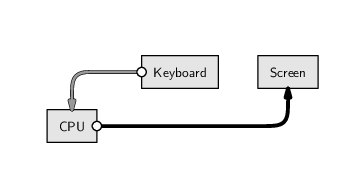
\includegraphics[width=0.5\linewidth]{img/script-commandline} \end{center}

\begin{center}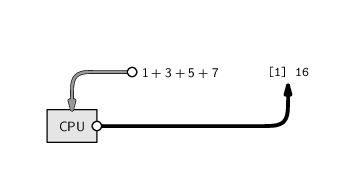
\includegraphics[width=0.5\linewidth]{img/script-commandlinedata} \end{center}

\begin{itemize}
\tightlist
\item
  Note que o resultado é apenas mostrado na tela, nada é salvo na
  memória (por enquanto)
\end{itemize}

\subsection{O editor de scripts}\label{o-editor-de-scripts}

\begin{itemize}
\tightlist
\item
  Para criar rotinas computacionais é necessário utilizar um editor de
  scripts.
\item
  Clique em
  \texttt{File\ \textgreater{}\ New\ file\ \textgreater{}\ R\ script}.
  Salve com a extensão \texttt{.R}.
\item
  Para enviar comandos diretamente para o console, selecione-os e aperte
  \texttt{Ctrl\ +\ \textless{}Enter\textgreater{}}.
\item
  Para adicionar comentários ao script, utiliza-se o símbolo \texttt{\#}
  antes do texto e/ou comandos. O que estiver depois do símbolo não será
  interpretado pelo R. Portanto:
\end{itemize}

\begin{Shaded}
\begin{Highlighting}[]
\DecValTok{2} \OperatorTok{+}\StringTok{ }\DecValTok{2}     \CommentTok{# esta linha será executada}
\CommentTok{# 2 + 2     esta linha não será executada}
\end{Highlighting}
\end{Shaded}

\subsection{Operadores aritméticos}\label{operadores-aritmeticos}

\begin{longtable}[]{@{}ll@{}}
\toprule
Operador & Significado\tabularnewline
\midrule
\endhead
\texttt{+} & adição\tabularnewline
\texttt{-} & subtração\tabularnewline
\texttt{*} & multiplicação\tabularnewline
\texttt{/} & divisão\tabularnewline
\texttt{\^{}} & potência\tabularnewline
\texttt{exp()} & exponencial\tabularnewline
\texttt{sqrt()} & raíz quadrada\tabularnewline
\texttt{factorial()} & fatorial\tabularnewline
\texttt{log()}; \texttt{log2()}; \texttt{log10()} &
logaritmos\tabularnewline
\bottomrule
\end{longtable}

\subsection{Ordens de execução}\label{ordens-de-execucao}

As operações são realizadas sempre seguindo as prioridades:

\begin{enumerate}
\def\labelenumi{\arabic{enumi}.}
\tightlist
\item
  De dentro para fora de parênteses \texttt{()}
\item
  Multiplicação e divisão
\item
  Adição e subtração
\end{enumerate}

\begin{Shaded}
\begin{Highlighting}[]
\OperatorTok{>}\StringTok{ }\DecValTok{5} \OperatorTok{*}\StringTok{ }\DecValTok{2} \OperatorTok{-}\StringTok{ }\DecValTok{10} \OperatorTok{+}\StringTok{ }\DecValTok{7}
\NormalTok{[}\DecValTok{1}\NormalTok{] }\DecValTok{7}
\OperatorTok{>}\StringTok{ }\DecValTok{5} \OperatorTok{*}\StringTok{ }\DecValTok{2} \OperatorTok{-}\StringTok{ }\NormalTok{(}\DecValTok{10} \OperatorTok{+}\StringTok{ }\DecValTok{7}\NormalTok{)}
\NormalTok{[}\DecValTok{1}\NormalTok{] }\OperatorTok{-}\DecValTok{7}
\OperatorTok{>}\StringTok{ }\DecValTok{5} \OperatorTok{*}\StringTok{ }\NormalTok{(}\DecValTok{2} \OperatorTok{-}\StringTok{ }\DecValTok{10} \OperatorTok{+}\StringTok{ }\DecValTok{7}\NormalTok{)}
\NormalTok{[}\DecValTok{1}\NormalTok{] }\OperatorTok{-}\DecValTok{5}
\OperatorTok{>}\StringTok{ }\DecValTok{5} \OperatorTok{*}\StringTok{ }\NormalTok{(}\DecValTok{2} \OperatorTok{-}\StringTok{ }\NormalTok{(}\DecValTok{10} \OperatorTok{+}\StringTok{ }\DecValTok{7}\NormalTok{))}
\NormalTok{[}\DecValTok{1}\NormalTok{] }\OperatorTok{-}\DecValTok{75}
\end{Highlighting}
\end{Shaded}

\subsection*{Exercícios}\label{exercicios}


\begin{enumerate}
\def\labelenumi{\arabic{enumi}.}
\tightlist
\item
  Calcule a seguinte equação: \(32 + 16^2 - 25^3\)
\item
  Divida o resultado por \(345\)
\item
  Qual o resultado da expressão \(\frac{e^{-2} 2^{4} - 1}{4!}\)?
\item
  E do logaritmo desta expressão?
\end{enumerate}

\subsection{\texorpdfstring{``Salvando''
resultados}{Salvando resultados}}\label{salvando-resultados}

Do exercício anterior

\begin{Shaded}
\begin{Highlighting}[]
\OperatorTok{>}\StringTok{ }\NormalTok{x <-}\StringTok{ }\DecValTok{32} \OperatorTok{+}\StringTok{ }\DecValTok{16}\OperatorTok{^}\DecValTok{2} \OperatorTok{-}\StringTok{ }\DecValTok{25}\OperatorTok{^}\DecValTok{3}
\OperatorTok{>}\StringTok{ }\NormalTok{x}
\NormalTok{[}\DecValTok{1}\NormalTok{] }\OperatorTok{-}\DecValTok{15337}
\OperatorTok{>}\StringTok{ }\NormalTok{x}\OperatorTok{/}\DecValTok{345}
\NormalTok{[}\DecValTok{1}\NormalTok{] }\OperatorTok{-}\FloatTok{44.45507}
\OperatorTok{>}\StringTok{ }\NormalTok{(y <-}\StringTok{ }\NormalTok{(}\KeywordTok{exp}\NormalTok{(}\OperatorTok{-}\DecValTok{2}\NormalTok{) }\OperatorTok{*}\StringTok{ }\DecValTok{2}\OperatorTok{^}\DecValTok{4} \OperatorTok{-}\StringTok{ }\DecValTok{1}\NormalTok{)}\OperatorTok{/}\KeywordTok{factorial}\NormalTok{(}\DecValTok{4}\NormalTok{))}
\NormalTok{[}\DecValTok{1}\NormalTok{] }\FloatTok{0.04855686}
\OperatorTok{>}\StringTok{ }\KeywordTok{log}\NormalTok{(y)}
\NormalTok{[}\DecValTok{1}\NormalTok{] }\OperatorTok{-}\FloatTok{3.02502}
\end{Highlighting}
\end{Shaded}

Quando criamos uma variável (\texttt{x}, \texttt{y}), ela fica
armazenada \textbf{temporariamente} na memória RAM.

\begin{center}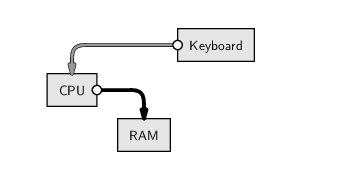
\includegraphics[width=0.5\linewidth]{img/script-assign} \end{center}

Para saber quais objetos estão criados, usamos a \textbf{função}
\texttt{ls()}

\begin{Shaded}
\begin{Highlighting}[]
\OperatorTok{>}\StringTok{ }\KeywordTok{ls}\NormalTok{()}
\NormalTok{[}\DecValTok{1}\NormalTok{] }\StringTok{"x"} \StringTok{"y"}
\end{Highlighting}
\end{Shaded}

Estas variáveis ficam armazenadas no chamado \emph{workspace} do R

\begin{itemize}
\tightlist
\item
  O \emph{workspace} consiste de tudo que or criado durante uma sessão
  do R, armazenado na memória RAM
\end{itemize}

Para efetivamente salvar esas variáveis, podemos armazenar esse
\emph{workspace} do R em disco, em um arquivo chamdo \texttt{.Rdata}

\begin{center}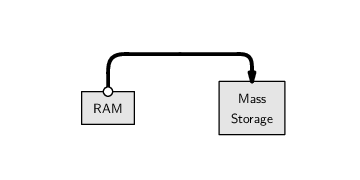
\includegraphics[width=0.5\linewidth]{img/script-workspace} \end{center}

\begin{center}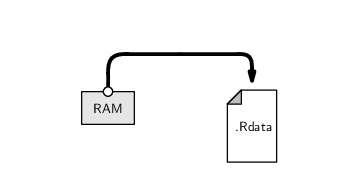
\includegraphics[width=0.5\linewidth]{img/script-workspacedata} \end{center}

\begin{itemize}
\tightlist
\item
  Quando o R é iniciado em um diretório com um arquivo \texttt{.Rdata},
  as variáveis salvas são automaticamente carregadas
\item
  No entanto, é sempre melhor salvar os dados e o \textbf{script}, assim
  é possível gerar os resultados novamente, sem salvar nada sem
  necessidade
\item
  Veremos mais pra frente como salvar variáveis específicas, por
  exemplo, resultados de uma análise que leva muito tempo para ser
  executada
\item
  O mais importante é salvar o \textbf{código}, assim sabemos
  \textbf{como} chegamos a determinado resultado, e podemos recriá-lo
  depois
\end{itemize}

\subsection{Finalizando o programa}\label{finalizando-o-programa}

A qualquer momento durante uma sessão você pode usar o comando

\begin{Shaded}
\begin{Highlighting}[]
\OperatorTok{>}\StringTok{ }\KeywordTok{save.image}\NormalTok{()}
\end{Highlighting}
\end{Shaded}

No RStudio:

\begin{itemize}
\tightlist
\item
  \texttt{File\ \textgreater{}\ Save\ As...}
\item
  Na janela que abrir, digite o nome do arquivo (por exemplo
  \texttt{script\_aula1}) e salve
\item
  Automaticamente o script será salvo com a extensão \texttt{.R} (nesse
  caso \texttt{script\_aula1.R}) no diretório de trabalho que você
  configurou no início
\end{itemize}

Alternativamente, você pode também salvar toda sua área de trabalho,
clicando em
\texttt{Workspace\ \textgreater{}\ Save\ As\ Default\ Workspace}. Este
processo irá gerar dois arquivos:

\begin{itemize}
\tightlist
\item
  \texttt{.Rdata}: contém todos os objetos criados durante uma sessão.
  Não é necessário (e nem recomendado) dar um nome antes do ponto. Dessa
  forma, a próxima vez que o programa for iniciado neste diretório, a
  área de trabalho será carregada automaticamente.
\item
  \texttt{.Rhistory}: um arquivo texto que contém todos os comandos que
  foram digitados no console.
\end{itemize}

\section*{Referências}\label{referencias}


\begin{itemize}
\tightlist
\item
  Leek, J. \href{https://leanpub.com/datastyle}{The Elements of Data
  Analytic Style}. Leanpub, 2015.
\item
  Murrell, P.
  \href{https://www.stat.auckland.ac.nz/~paul/ItDT/HTML}{Introduction to
  data technologies}. Boca Raton: Chapman \& Hall/CRC, 2009.
\item
  Peng, RD. \href{https://leanpub.com/rprogramming}{R programming for
  data science}. Leanpub, 2015.
\end{itemize}

\chapter{Objetos e classes}\label{objetos-e-classes}

\section{Funções e argumentos}\label{funcoes-e-argumentos}

As funções no R são definidas como:

\begin{Shaded}
\begin{Highlighting}[]
\KeywordTok{nome}\NormalTok{(argumento1, argumento2, ...)}
\end{Highlighting}
\end{Shaded}

Exemplo: função \texttt{runif()} (para gerar valores aleatórios de uma
distribuição uniforme):

\begin{Shaded}
\begin{Highlighting}[]
\KeywordTok{runif}\NormalTok{(n, }\DataTypeTok{min =} \DecValTok{0}\NormalTok{, }\DataTypeTok{max =} \DecValTok{1}\NormalTok{)}
\end{Highlighting}
\end{Shaded}

\begin{Shaded}
\begin{Highlighting}[]
\KeywordTok{runif}\NormalTok{(}\DecValTok{10}\NormalTok{, }\DecValTok{1}\NormalTok{, }\DecValTok{100}\NormalTok{)}
\NormalTok{ [}\DecValTok{1}\NormalTok{] }\FloatTok{31.468845} \FloatTok{26.509578} \FloatTok{55.679921}  \FloatTok{6.581932} \FloatTok{47.386379} \FloatTok{48.893303} \FloatTok{81.427859}
\NormalTok{ [}\DecValTok{8}\NormalTok{] }\FloatTok{37.661733} \FloatTok{55.109301} \FloatTok{17.855943}
\end{Highlighting}
\end{Shaded}

Argumentos que já possuem um valor especificado (como \texttt{max} e
\texttt{min}) podem ser omitidos:

\begin{Shaded}
\begin{Highlighting}[]
\KeywordTok{runif}\NormalTok{(}\DecValTok{10}\NormalTok{)}
\end{Highlighting}
\end{Shaded}

Se os argumentos forem nomeados, a ordem deles dentro da função não tem
mais importância:

\begin{Shaded}
\begin{Highlighting}[]
\KeywordTok{runif}\NormalTok{(}\DataTypeTok{min =} \DecValTok{1}\NormalTok{, }\DataTypeTok{max =} \DecValTok{100}\NormalTok{, }\DataTypeTok{n =} \DecValTok{10}\NormalTok{)}
\end{Highlighting}
\end{Shaded}

Argumentos nomeados e não nomeados podem ser utilizados, desde que os
não nomeados estejam na posição correta:

\begin{Shaded}
\begin{Highlighting}[]
\KeywordTok{runif}\NormalTok{(}\DecValTok{10}\NormalTok{, }\DataTypeTok{max =} \DecValTok{100}\NormalTok{, }\DataTypeTok{min =} \DecValTok{1}\NormalTok{)}
\end{Highlighting}
\end{Shaded}

\subsection{Outros tipos de
argumentos}\label{outros-tipos-de-argumentos}

Exemplo: função \texttt{sample()}:

\begin{Shaded}
\begin{Highlighting}[]
\KeywordTok{sample}\NormalTok{(x, size, }\DataTypeTok{replace =} \OtherTok{FALSE}\NormalTok{, }\DataTypeTok{prob =} \OtherTok{NULL}\NormalTok{)}
\end{Highlighting}
\end{Shaded}

\begin{itemize}
\tightlist
\item
  \texttt{x} e \texttt{size} devem ser obrigatoriamente especificados
\item
  \texttt{replace} é lógico: \texttt{TRUE} (\texttt{T}) ou
  \texttt{FALSE} (\texttt{F})
\item
  \texttt{prob} é um argumento vazio ou ausente (``opcional'')
\end{itemize}

Exemplo: função \texttt{plot()}:

\begin{Shaded}
\begin{Highlighting}[]
\KeywordTok{plot}\NormalTok{(x, y, ...)}
\end{Highlighting}
\end{Shaded}

\begin{itemize}
\tightlist
\item
  ``\texttt{...}'' permite especificar argumentos de outras funções (por
  exemplo \texttt{par()})
\end{itemize}

Para ver todos os argumentos disponíveis de uma função, podemos usar a
função \texttt{args()}

\begin{Shaded}
\begin{Highlighting}[]
\KeywordTok{args}\NormalTok{(sample)}
\ControlFlowTok{function}\NormalTok{ (x, size, }\DataTypeTok{replace =} \OtherTok{FALSE}\NormalTok{, }\DataTypeTok{prob =} \OtherTok{NULL}\NormalTok{) }
\OtherTok{NULL}
\end{Highlighting}
\end{Shaded}

\section{Mecanismos de ajuda}\label{mecanismos-de-ajuda}

Argumentos e detalhes do funcionamento das funções:

\begin{Shaded}
\begin{Highlighting}[]
\NormalTok{?runif}
\end{Highlighting}
\end{Shaded}

ou

\begin{Shaded}
\begin{Highlighting}[]
\KeywordTok{help}\NormalTok{(runif)}
\end{Highlighting}
\end{Shaded}

A documentação contém os campos:

\begin{itemize}
\tightlist
\item
  \textbf{Description:} breve descrição
\item
  \textbf{Usage:} função e todos seus argumentos
\item
  \textbf{Arguments:} lista descrevendo cada argumento
\item
  \textbf{Details:} descrição detalhada
\item
  \textbf{Value:} o que a função retorna
\item
  \textbf{References:} bibliografia relacionada
\item
  \textbf{See Also:} funções relacionadas
\item
  \textbf{Examples:} exemplos práticos
\end{itemize}

Procura por nomes de funções que contenham algum termo:

\begin{Shaded}
\begin{Highlighting}[]
\KeywordTok{apropos}\NormalTok{(}\StringTok{"mod"}\NormalTok{)}
\KeywordTok{apropos}\NormalTok{(}\StringTok{"model"}\NormalTok{)}
\end{Highlighting}
\end{Shaded}

Procura por funções que contenham \texttt{palavra} em qualquer parte de
sua documentação:

\begin{Shaded}
\begin{Highlighting}[]
\KeywordTok{help.search}\NormalTok{(}\StringTok{"palavra"}\NormalTok{)}
\end{Highlighting}
\end{Shaded}

Ajuda através do navegador (também contém manuais, \ldots{}):

\begin{Shaded}
\begin{Highlighting}[]
\KeywordTok{help.start}\NormalTok{()}
\end{Highlighting}
\end{Shaded}

Sites para busca na documentação dos diversos pacotes:

\begin{itemize}
\tightlist
\item
  RDocumentation \url{https://www.rdocumentation.org/}
\item
  R Package Documentation \url{https://rdrr.io/}
\item
  R Contributed Documentation (várias línguas)
  \url{https://cran.r-project.org/other-docs.html}
\end{itemize}

Os pacotes do R contém funções específicas para determinadas tarefas, e
estendem a instalação básica do R. Atualmente existem mais de 10000
pacotes disponíveis no
\href{http://cran-r.c3sl.ufpr.br/web/packages/index.html}{CRAN}, além de
diversos outros hospedados em sites como
\href{https://github.com}{Github}, por exemplo.

Ao instalar o R, os seguintes pacotes já vêm instalados (fazem parte do
chamado ``R core''):

\begin{verbatim}
NULL
\end{verbatim}

No entanto, nem todos são carregados na inicialização do R. Por padrão,
apenas os seguintes pacotes são carregados automaticamente:

\begin{verbatim}
[1] "graphics"  "grDevices" "utils"     "datasets"  "methods"   "base"     
\end{verbatim}

Para listar os pacotes carregados, use a função

\begin{Shaded}
\begin{Highlighting}[]
\KeywordTok{search}\NormalTok{()}
\end{Highlighting}
\end{Shaded}

Note que o primeiro elemento, \texttt{.GlobalEnv}, será sempre carregado
pois ele é o \emph{ambiente} queirá armazenar (e deixar disponível) os
objetos criados pelo usuário. Para carregar um pacote instalado, usamos
a função \texttt{library()}, por exemplo

\begin{Shaded}
\begin{Highlighting}[]
\KeywordTok{library}\NormalTok{(lattice)}
\KeywordTok{search}\NormalTok{()}
\end{Highlighting}
\end{Shaded}

Isso tornará todas as funções do pacote \texttt{lattice} disponíveis
para uso.

Para instalar um pacote usamos a função \texttt{install.packages()}.
Sabendo o nome do pacote, por exemplo, \texttt{mvtnorm}, fazemos

\begin{Shaded}
\begin{Highlighting}[]
\KeywordTok{install.packages}\NormalTok{(}\StringTok{"mvtnorm"}\NormalTok{)}
\end{Highlighting}
\end{Shaded}

Se o diretório padrão de instalação de um pacote for de acesso restrito
(root por exemplo), o R irá perguntar se você gostaria de instalar o
pacote em uma biblioteca pessoal, e sugerirá um diretório que possui as
permissões necessárias. Você pode se antecipar e já definir e criar um
diretório na sua pasta pessoal, e instalar os pacotes sempre nesse
local. Por exemplo, defina \texttt{\textasciitilde{}/R/library} como sua
biblioteca pessoal. Para instalar os pacotes sempre nesse diretório
faça:

\begin{Shaded}
\begin{Highlighting}[]
\KeywordTok{install.packages}\NormalTok{(}\StringTok{"mvtnorm"}\NormalTok{, }\DataTypeTok{lib =} \StringTok{"~/R/library"}\NormalTok{)}
\end{Highlighting}
\end{Shaded}

Para verificar as bibliotecas disponíveis e se existem pacotes para ser
atualizados, use

\begin{Shaded}
\begin{Highlighting}[]
\KeywordTok{packageStatus}\NormalTok{()}
\end{Highlighting}
\end{Shaded}

Para atualizar automaticamente todos os pacotes faça

\begin{Shaded}
\begin{Highlighting}[]
\KeywordTok{update.packages}\NormalTok{(}\DataTypeTok{ask =} \OtherTok{FALSE}\NormalTok{)}
\end{Highlighting}
\end{Shaded}

\section{Criando uma função}\label{criando-uma-funcao}

A ideia original do R é transformar usuários em programadores

\begin{quote}
\emph{``\ldots{} to turn ideas into software, quickly and faithfully.''}

-- John M. Chambers
\end{quote}

Criar funções para realizar trabalhos específicos é um dos grandes
poderes do R

Por exemplo, podemos criar a famosa função

\begin{Shaded}
\begin{Highlighting}[]
\NormalTok{ola.mundo <-}\StringTok{ }\ControlFlowTok{function}\NormalTok{()\{}
    \KeywordTok{writeLines}\NormalTok{(}\StringTok{"Olá mundo"}\NormalTok{)}
\NormalTok{\}}
\end{Highlighting}
\end{Shaded}

E chama-la através de

\begin{Shaded}
\begin{Highlighting}[]
\KeywordTok{ola.mundo}\NormalTok{()}
\NormalTok{Olá mundo}
\end{Highlighting}
\end{Shaded}

A função acima não permite alterar o resultado de saída. Podemos fazer
isso incluindo um \textbf{argumento}

\begin{Shaded}
\begin{Highlighting}[]
\NormalTok{ola.mundo <-}\StringTok{ }\ControlFlowTok{function}\NormalTok{(texto)\{}
    \KeywordTok{writeLines}\NormalTok{(texto)}
\NormalTok{\}}
\end{Highlighting}
\end{Shaded}

E fazer por exemplo

\begin{Shaded}
\begin{Highlighting}[]
\KeywordTok{ola.mundo}\NormalTok{(}\StringTok{"Funções são legais"}\NormalTok{)}
\NormalTok{Funções são legais}
\end{Highlighting}
\end{Shaded}

(Veremos detalhes de funções mais adiante)

\section*{Exercícios}\label{exercicios-1}


\begin{enumerate}
\def\labelenumi{\arabic{enumi}.}
\tightlist
\item
  Usando a função \texttt{runif()} gere \(30\) números aleatórios entre:

  \begin{itemize}
  \tightlist
  \item
    0 e 1
  \item
    -5 e 5
  \item
    10 e 500
  \end{itemize}
\end{enumerate}

alternando a posição dos argumentos da função.

\begin{enumerate}
\def\labelenumi{\arabic{enumi}.}
\setcounter{enumi}{1}
\tightlist
\item
  Veja o help da função (?) \texttt{"+"}
\item
  Crie uma função para fazer a soma de dois números: \texttt{x} e
  \texttt{y}
\item
  Crie uma função para simular a jogada de um dado.
\item
  Crie uma função para simular a jogada de dois dados.
\end{enumerate}

\section{Objetos}\label{objetos}

O que é um objeto?

\begin{itemize}
\tightlist
\item
  Um \textbf{símbolo} ou uma \textbf{variável} capaz de armazenar
  qualquer valor ou estrutura de dados
\end{itemize}

Por quê objetos?

\begin{itemize}
\tightlist
\item
  Uma maneira simples de acessar os dados armazenados na memória (o R
  não permite acesso direto à memória)
\end{itemize}

Programação:

\begin{itemize}
\tightlist
\item
  Objetos \(\Rightarrow\) Classes \(\Rightarrow\) Métodos
\end{itemize}

\begin{quote}
\emph{``Tudo no R é um objeto.''}
\end{quote}

\begin{quote}
\emph{``Todo objeto no R tem uma classe''}
\end{quote}

\begin{itemize}
\tightlist
\item
  \textbf{Classe:} é a definição de um objeto. Descreve a forma do
  objeto e como ele será manipulado pelas diferentes funções
\item
  \textbf{Método:} são \textbf{funções genéricas} que executam suas
  tarefas de acordo com cada classe. Duas das funções genéricas mais
  importantes são:

  \begin{itemize}
  \tightlist
  \item
    \texttt{summary()}
  \item
    \texttt{plot()}
  \end{itemize}
\end{itemize}

Veja o resultado de

\begin{Shaded}
\begin{Highlighting}[]
\KeywordTok{methods}\NormalTok{(summary)}
\KeywordTok{methods}\NormalTok{(plot)}
\end{Highlighting}
\end{Shaded}

(Veremos mais detalhes adiante).

A variável \texttt{x} recebe o valor \(2\) (tornando-se um objeto dentro
do R):

\begin{Shaded}
\begin{Highlighting}[]
\NormalTok{x <-}\StringTok{ }\DecValTok{2}
\end{Highlighting}
\end{Shaded}

O símbolo \texttt{\textless{}-} é chamado de \textbf{operador de
atribuição}. Ele serve para atribuir valores a objetos, e é formado
pelos símbolos \texttt{\textless{}} e \texttt{-}, obrigatoriamente
\textbf{sem espaços}.

Para ver o conteúdo do objeto:

\begin{Shaded}
\begin{Highlighting}[]
\NormalTok{x}
\NormalTok{[}\DecValTok{1}\NormalTok{] }\DecValTok{2}
\end{Highlighting}
\end{Shaded}

\textbf{Observação}: O símbolo \texttt{=} pode ser usado no lugar de
\texttt{\textless{}-} mas não é recomendado.

Quando você faz

\begin{Shaded}
\begin{Highlighting}[]
\NormalTok{x <-}\StringTok{ }\DecValTok{2}
\end{Highlighting}
\end{Shaded}

está fazendo uma \textbf{declaração}, ou seja, declarando que a variável
\texttt{x} irá agora se tornar um objeto que armazena o número
\texttt{2}. As declarações podem ser feitas uma em cada linha

\begin{Shaded}
\begin{Highlighting}[]
\NormalTok{x <-}\StringTok{ }\DecValTok{2}
\NormalTok{y <-}\StringTok{ }\DecValTok{4}
\end{Highlighting}
\end{Shaded}

ou separadas por \texttt{;}

\begin{Shaded}
\begin{Highlighting}[]
\NormalTok{x <-}\StringTok{ }\DecValTok{2}\NormalTok{; y <-}\StringTok{ }\DecValTok{4}
\end{Highlighting}
\end{Shaded}

Operações matemáticas em objetos:

\begin{Shaded}
\begin{Highlighting}[]
\NormalTok{x }\OperatorTok{+}\StringTok{ }\NormalTok{x}
\NormalTok{[}\DecValTok{1}\NormalTok{] }\DecValTok{4}
\end{Highlighting}
\end{Shaded}

Objetos podem armazenar diferentes estruturas de dados:

\begin{Shaded}
\begin{Highlighting}[]
\NormalTok{y <-}\StringTok{ }\KeywordTok{runif}\NormalTok{(}\DecValTok{10}\NormalTok{)}
\NormalTok{y}
\NormalTok{ [}\DecValTok{1}\NormalTok{] }\FloatTok{0.6249965} \FloatTok{0.8821655} \FloatTok{0.2803538} \FloatTok{0.3984879} \FloatTok{0.7625511} \FloatTok{0.6690217} \FloatTok{0.2046122}
\NormalTok{ [}\DecValTok{8}\NormalTok{] }\FloatTok{0.3575249} \FloatTok{0.3594751} \FloatTok{0.6902905}
\end{Highlighting}
\end{Shaded}

Note que cada objeto só pode armazenar uma estrutura (um número ou uma
sequência de valores) de cada vez! (Aqui, o valor \(4\) que estava
armazenado em \texttt{y} foi sobrescrito pelos valores acima.)

\subsection{Nomes de objetos}\label{nomes-de-objetos}

\begin{itemize}
\tightlist
\item
  Podem ser formados por letras, números, ``\texttt{\_}'', e
  ``\texttt{.}''
\item
  Não podem começar com número e/ou ponto
\item
  Não podem conter espaços
\item
  Evite usar acentos
\item
  Evite usar nomes de funções como:
\end{itemize}

\texttt{c\ q\ t\ C\ D\ F\ I\ T\ diff\ df\ data\ var\ pt}

\begin{itemize}
\tightlist
\item
  O R é \emph{case-sensitive}, portanto:
\end{itemize}

\texttt{dados} \(\neq\) \texttt{Dados} \(\neq\) \texttt{DADOS}

\subsection{Gerenciando a área de
trabalho}\label{gerenciando-a-area-de-trabalho}

Liste os objetos criados com a função \texttt{ls()}:

\begin{Shaded}
\begin{Highlighting}[]
\KeywordTok{ls}\NormalTok{()}
\end{Highlighting}
\end{Shaded}

Para remover apenas um objeto:

\begin{Shaded}
\begin{Highlighting}[]
\KeywordTok{rm}\NormalTok{(x)}
\end{Highlighting}
\end{Shaded}

Para remover outros objetos:

\begin{Shaded}
\begin{Highlighting}[]
\KeywordTok{rm}\NormalTok{(x, y)}
\end{Highlighting}
\end{Shaded}

Para remover todos os objetos:

\begin{Shaded}
\begin{Highlighting}[]
\KeywordTok{rm}\NormalTok{(}\DataTypeTok{list =} \KeywordTok{ls}\NormalTok{())}
\end{Highlighting}
\end{Shaded}

\textbf{Cuidado!} O comando acima apaga todos os objetos na sua área de
trabalho sem perguntar. Depois só é possível recuperar os objetos ao
rodar os script novamente.

\section*{Exercícios}\label{exercicios-2}


\begin{enumerate}
\def\labelenumi{\arabic{enumi}.}
\tightlist
\item
  Armazene o resultado da equação \(32 + 16^2 - 25^3\) no objeto
  \texttt{x}
\item
  Divida \texttt{x} por \(345\) e armazene em \texttt{y}
\item
  Crie um objeto (com o nome que você quiser) para armazenar \(30\)
  valores aleatórios de uma distribuição uniforme entre \(10\) e \(50\)
\item
  Remova o objeto \texttt{y}
\item
  Remova os demais objetos de uma única vez
\item
  Procure a função utilizada para gerar numeros aleatórios de uma
  distribuição de Poisson, e gere \(100\) valores para a VA
  \(X \sim  \text{Poisson}(5)\).
\end{enumerate}

\section{Tipos e classes de objetos}\label{tipos-e-classes-de-objetos}

Para saber como trabalhar com dados no R, é fundamental entender as
possíveis estruturas (ou tipos) de dados possíveis. O formato mais
básico de dados são os vetores, e a partir deles, outras estruturas mais
complexas podem ser construídas. O R possui dois tipos básicos de
vetores:

\begin{itemize}
\tightlist
\item
  \textbf{Vetores atômicos}: existem seis tipos básicos:
\item
  \texttt{double}
\item
  \texttt{integer}
\item
  \texttt{character}
\item
  \texttt{logical}
\item
  \texttt{complex}
\item
  \texttt{raw}
\end{itemize}

Os tipos \texttt{integer} e \texttt{double} são chamados conjuntamente
de \texttt{numeric}. - \textbf{Listas}: também chamadas de \emph{vetores
recursivos} pois listas podem conter outras listas.

A principal diferença entre vetores atômicos e listas é que o primeiro é
\textbf{homogêneo} (cada vetor só pode conter um tipo), enquanto que o
segundo pode ser \textbf{heterogêneo} (cada vetor pode conter mais de um
tipo).

Um vetor atômico só pode conter elementos de um mesmo tipo

Um vetor, como o próprio nome diz, é uma estrutura unidimensional, mas
na maioria das vezes iremos trabalhar com estruturas de dados
bidimensionais (linhas e colunas). Portanto diferentes estruturas (com
diferentes dimensões) podem ser criadas a partir dos vetores atômicos.
Quando isso acontece, temos o que é chamado de \textbf{classe} de um
objeto. Embora os vetores atômicos só possuam seis tipos básicos, existe
um número muito grande de classes, e novas são inventadas todos os dias.
E mesmo que um objeto seja de qualquer classe, ele sempre será de um dos
seis tipos básicos (ou uma lista).

Para verificar o tipo de um objeto, usamos a função \texttt{typeof()},
enquanto que a classe é verificada com a função \texttt{class()}.
Vejamos alguns exemplos:

\begin{Shaded}
\begin{Highlighting}[]
\NormalTok{## double}
\NormalTok{x <-}\StringTok{ }\KeywordTok{c}\NormalTok{(}\DecValTok{2}\NormalTok{, }\DecValTok{4}\NormalTok{, }\DecValTok{6}\NormalTok{)}
\KeywordTok{typeof}\NormalTok{(x)}
\NormalTok{[}\DecValTok{1}\NormalTok{] }\StringTok{"double"}
\KeywordTok{class}\NormalTok{(x)}
\NormalTok{[}\DecValTok{1}\NormalTok{] }\StringTok{"numeric"}
\NormalTok{## integer}
\NormalTok{x <-}\StringTok{ }\KeywordTok{c}\NormalTok{(2L, 4L, 6L)}
\KeywordTok{typeof}\NormalTok{(x)}
\NormalTok{[}\DecValTok{1}\NormalTok{] }\StringTok{"integer"}
\KeywordTok{class}\NormalTok{(x)}
\NormalTok{[}\DecValTok{1}\NormalTok{] }\StringTok{"integer"}
\NormalTok{## character}
\NormalTok{x <-}\StringTok{ }\KeywordTok{c}\NormalTok{(}\StringTok{"a"}\NormalTok{, }\StringTok{"b"}\NormalTok{, }\StringTok{"c"}\NormalTok{)}
\KeywordTok{typeof}\NormalTok{(x)}
\NormalTok{[}\DecValTok{1}\NormalTok{] }\StringTok{"character"}
\KeywordTok{class}\NormalTok{(x)}
\NormalTok{[}\DecValTok{1}\NormalTok{] }\StringTok{"character"}
\NormalTok{## logical}
\NormalTok{x <-}\StringTok{ }\KeywordTok{c}\NormalTok{(}\OtherTok{TRUE}\NormalTok{, }\OtherTok{FALSE}\NormalTok{, }\OtherTok{TRUE}\NormalTok{)}
\KeywordTok{typeof}\NormalTok{(x)}
\NormalTok{[}\DecValTok{1}\NormalTok{] }\StringTok{"logical"}
\KeywordTok{class}\NormalTok{(x)}
\NormalTok{[}\DecValTok{1}\NormalTok{] }\StringTok{"logical"}
\NormalTok{## complex}
\NormalTok{x <-}\StringTok{ }\KeywordTok{c}\NormalTok{(}\DecValTok{2} \OperatorTok{+}\StringTok{ }\NormalTok{1i, }\DecValTok{4} \OperatorTok{+}\StringTok{ }\NormalTok{1i, }\DecValTok{6} \OperatorTok{+}\StringTok{ }\NormalTok{1i)}
\KeywordTok{typeof}\NormalTok{(x)}
\NormalTok{[}\DecValTok{1}\NormalTok{] }\StringTok{"complex"}
\KeywordTok{class}\NormalTok{(x)}
\NormalTok{[}\DecValTok{1}\NormalTok{] }\StringTok{"complex"}
\NormalTok{## raw}
\NormalTok{x <-}\StringTok{ }\KeywordTok{raw}\NormalTok{(}\DecValTok{3}\NormalTok{)}
\KeywordTok{typeof}\NormalTok{(x)}
\NormalTok{[}\DecValTok{1}\NormalTok{] }\StringTok{"raw"}
\KeywordTok{class}\NormalTok{(x)}
\NormalTok{[}\DecValTok{1}\NormalTok{] }\StringTok{"raw"}
\end{Highlighting}
\end{Shaded}

\subsection{Vetores numéricos}\label{vetores-numericos}

Características:

\begin{itemize}
\tightlist
\item
  Coleção ordenada de valores
\item
  Estrutura unidimensional
\end{itemize}

Usando a função \texttt{c()} para criar vetores:

\begin{Shaded}
\begin{Highlighting}[]
\NormalTok{num <-}\StringTok{ }\KeywordTok{c}\NormalTok{(}\DecValTok{10}\NormalTok{, }\DecValTok{5}\NormalTok{, }\DecValTok{2}\NormalTok{, }\DecValTok{4}\NormalTok{, }\DecValTok{8}\NormalTok{, }\DecValTok{9}\NormalTok{)}
\NormalTok{num}
\NormalTok{[}\DecValTok{1}\NormalTok{] }\DecValTok{10}  \DecValTok{5}  \DecValTok{2}  \DecValTok{4}  \DecValTok{8}  \DecValTok{9}
\KeywordTok{typeof}\NormalTok{(num)}
\NormalTok{[}\DecValTok{1}\NormalTok{] }\StringTok{"double"}
\KeywordTok{class}\NormalTok{(num)}
\NormalTok{[}\DecValTok{1}\NormalTok{] }\StringTok{"numeric"}
\end{Highlighting}
\end{Shaded}

Por que \texttt{numeric} e não \texttt{integer}?

\begin{Shaded}
\begin{Highlighting}[]
\NormalTok{x <-}\StringTok{ }\KeywordTok{c}\NormalTok{(10L, 5L, 2L, 4L, 8L, 9L)}
\NormalTok{x}
\NormalTok{[}\DecValTok{1}\NormalTok{] }\DecValTok{10}  \DecValTok{5}  \DecValTok{2}  \DecValTok{4}  \DecValTok{8}  \DecValTok{9}
\KeywordTok{typeof}\NormalTok{(x)}
\NormalTok{[}\DecValTok{1}\NormalTok{] }\StringTok{"integer"}
\KeywordTok{class}\NormalTok{(x)}
\NormalTok{[}\DecValTok{1}\NormalTok{] }\StringTok{"integer"}
\end{Highlighting}
\end{Shaded}

Para forçar a representação de um número para inteiro é necessário usar
o sufixo \texttt{L}.

Note que a diferença entre \texttt{numeric} e \texttt{integer} também
possui impacto computacional, pois o armazenamento de números inteiros
ocupa menos espaço na memória. Dessa forma, esperamos que o vetor
\texttt{x} acima ocupe menos espaço na memória do que o vetor
\texttt{num}, embora sejam aparentemente idênticos. Veja:

\begin{Shaded}
\begin{Highlighting}[]
\KeywordTok{object.size}\NormalTok{(num)}
\DecValTok{96}\NormalTok{ bytes}
\KeywordTok{object.size}\NormalTok{(x)}
\DecValTok{80}\NormalTok{ bytes}
\end{Highlighting}
\end{Shaded}

A diferença pode parecer pequena, mas pode ter um grande impacto
computacional quando os vetores são formados por milhares ou milhões de
números.

\subsubsection{Representação numérica dentro do
R}\label{representacao-numerica-dentro-do-r}

Os números que aparecem na tela do console do R são apenas
representações simplificadas do número real armazenado na memória. Por
exemplo,

\begin{Shaded}
\begin{Highlighting}[]
\NormalTok{x <-}\StringTok{ }\KeywordTok{runif}\NormalTok{(}\DecValTok{10}\NormalTok{)}
\NormalTok{x}
\NormalTok{ [}\DecValTok{1}\NormalTok{] }\FloatTok{0.2875775} \FloatTok{0.7883051} \FloatTok{0.4089769} \FloatTok{0.8830174} \FloatTok{0.9404673} \FloatTok{0.0455565} \FloatTok{0.5281055}
\NormalTok{ [}\DecValTok{8}\NormalTok{] }\FloatTok{0.8924190} \FloatTok{0.5514350} \FloatTok{0.4566147}
\end{Highlighting}
\end{Shaded}

O objeto \texttt{x} contém números como 0.2875775, 0.7883051, etc, que
possuem 7 casas decimais, que é o padrão do R. O número de casas
decimais é controlado pelo argumento \texttt{digits} da função
\texttt{options()}. Para visualizar essa opção, use

\begin{Shaded}
\begin{Highlighting}[]
\KeywordTok{getOption}\NormalTok{(}\StringTok{"digits"}\NormalTok{)}
\NormalTok{[}\DecValTok{1}\NormalTok{] }\DecValTok{7}
\end{Highlighting}
\end{Shaded}

Note que esse valor de 7 é o número de \textbf{dígitos significativos},
e pode variar conforme a sequência de números. Por exemplo,

\begin{Shaded}
\begin{Highlighting}[]
\NormalTok{y <-}\StringTok{ }\KeywordTok{runif}\NormalTok{(}\DecValTok{10}\NormalTok{)}
\NormalTok{y}
\NormalTok{ [}\DecValTok{1}\NormalTok{] }\FloatTok{0.069360916} \FloatTok{0.817775199} \FloatTok{0.942621732} \FloatTok{0.269381876} \FloatTok{0.169348123}
\NormalTok{ [}\DecValTok{6}\NormalTok{] }\FloatTok{0.033895622} \FloatTok{0.178785004} \FloatTok{0.641665366} \FloatTok{0.022877743} \FloatTok{0.008324827}
\end{Highlighting}
\end{Shaded}

possui valores com 9 casas decimais. Isto é apenas a representação do
número que aparece na tela. Internamente, cada número é armazenado com
uma precisão de 64 bits. Como consequência, cada número possui uma
acurácia de até 16 dígitos significativos. Isso pode introduzir algum
tipo de erro, por exemplo:

\begin{Shaded}
\begin{Highlighting}[]
\KeywordTok{sqrt}\NormalTok{(}\DecValTok{2}\NormalTok{)}\OperatorTok{^}\DecValTok{2} \OperatorTok{-}\StringTok{ }\DecValTok{2}
\NormalTok{[}\DecValTok{1}\NormalTok{] }\FloatTok{4.440892e-16}
\KeywordTok{print}\NormalTok{(}\KeywordTok{sqrt}\NormalTok{(}\DecValTok{2}\NormalTok{)}\OperatorTok{^}\DecValTok{2}\NormalTok{, }\DataTypeTok{digits =} \DecValTok{22}\NormalTok{)}
\NormalTok{[}\DecValTok{1}\NormalTok{] }\FloatTok{2.000000000000000444089}
\end{Highlighting}
\end{Shaded}

não é exatamente zero, pois a raíz quadrada de 2 não pode ser armazenada
com toda precisão com ``apenas'' 16 dígitos significativos. Esse tipo de
erro é chamado de \textbf{erro de ponto flutuante}, e as operações
nessas condições são chamadas de \textbf{aritmética de ponto flutuante}.
Para mais informações sobre esse assunto veja
\href{http://www.validlab.com/goldberg/paper.pdf}{What Every Computer
Scientist Should Know About Floating-Point Arithmetic} e
\href{http://cran-r.c3sl.ufpr.br/doc/FAQ/R-FAQ.html\#Why-doesn_0027t-R-think-these-numbers-are-equal_003f}{Why
doesn't R think these numbers are equal?}.

No R os números podem ser representados com até 22 casas decimais. Você
pode ver o número com toda sua precisão usando a função \texttt{print()}
e especificando o número de casas decimais com o argumento
\texttt{digits} (de 1 a 22)

\begin{Shaded}
\begin{Highlighting}[]
\KeywordTok{print}\NormalTok{(x, }\DataTypeTok{digits =} \DecValTok{1}\NormalTok{)}
\NormalTok{ [}\DecValTok{1}\NormalTok{] }\FloatTok{0.29} \FloatTok{0.79} \FloatTok{0.41} \FloatTok{0.88} \FloatTok{0.94} \FloatTok{0.05} \FloatTok{0.53} \FloatTok{0.89} \FloatTok{0.55} \FloatTok{0.46}
\KeywordTok{print}\NormalTok{(x, }\DataTypeTok{digits =} \DecValTok{7}\NormalTok{) }\CommentTok{# padrão}
\NormalTok{ [}\DecValTok{1}\NormalTok{] }\FloatTok{0.2875775} \FloatTok{0.7883051} \FloatTok{0.4089769} \FloatTok{0.8830174} \FloatTok{0.9404673} \FloatTok{0.0455565} \FloatTok{0.5281055}
\NormalTok{ [}\DecValTok{8}\NormalTok{] }\FloatTok{0.8924190} \FloatTok{0.5514350} \FloatTok{0.4566147}
\KeywordTok{print}\NormalTok{(x, }\DataTypeTok{digits =} \DecValTok{22}\NormalTok{)}
\NormalTok{ [}\DecValTok{1}\NormalTok{] }\FloatTok{0.28757752012461423873901} \FloatTok{0.78830513544380664825439}
\NormalTok{ [}\DecValTok{3}\NormalTok{] }\FloatTok{0.40897692181169986724854} \FloatTok{0.88301740400493144989014}
\NormalTok{ [}\DecValTok{5}\NormalTok{] }\FloatTok{0.94046728429384529590607} \FloatTok{0.04555649938993155956268}
\NormalTok{ [}\DecValTok{7}\NormalTok{] }\FloatTok{0.52810548804700374603271} \FloatTok{0.89241904439404606819153}
\NormalTok{ [}\DecValTok{9}\NormalTok{] }\FloatTok{0.55143501446582376956940} \FloatTok{0.45661473530344665050507}
\end{Highlighting}
\end{Shaded}

Também é possível alterar a representação na tela para o formato
científico, usando a função \texttt{format()}

\begin{Shaded}
\begin{Highlighting}[]
\KeywordTok{format}\NormalTok{(x, }\DataTypeTok{scientific =} \OtherTok{TRUE}\NormalTok{)}
\NormalTok{ [}\DecValTok{1}\NormalTok{] }\StringTok{"2.875775e-01"} \StringTok{"7.883051e-01"} \StringTok{"4.089769e-01"} \StringTok{"8.830174e-01"}
\NormalTok{ [}\DecValTok{5}\NormalTok{] }\StringTok{"9.404673e-01"} \StringTok{"4.555650e-02"} \StringTok{"5.281055e-01"} \StringTok{"8.924190e-01"}
\NormalTok{ [}\DecValTok{9}\NormalTok{] }\StringTok{"5.514350e-01"} \StringTok{"4.566147e-01"}
\end{Highlighting}
\end{Shaded}

Nessa representação, o valor 2.875775e-01 = \(2.875775 \times 10^{-01}\)
= \(0.2875775\).

\subsubsection{Sequências de números}\label{sequencias-de-numeros}

Usando a função \texttt{seq()}

\begin{Shaded}
\begin{Highlighting}[]
\KeywordTok{seq}\NormalTok{(}\DecValTok{1}\NormalTok{, }\DecValTok{10}\NormalTok{)}
\NormalTok{ [}\DecValTok{1}\NormalTok{]  }\DecValTok{1}  \DecValTok{2}  \DecValTok{3}  \DecValTok{4}  \DecValTok{5}  \DecValTok{6}  \DecValTok{7}  \DecValTok{8}  \DecValTok{9} \DecValTok{10}
\end{Highlighting}
\end{Shaded}

Ou \texttt{1:10} gera o mesmo resultado. Para a sequência variar em
\(2\)

\begin{Shaded}
\begin{Highlighting}[]
\KeywordTok{seq}\NormalTok{(}\DataTypeTok{from =} \DecValTok{1}\NormalTok{, }\DataTypeTok{to =} \DecValTok{10}\NormalTok{, }\DataTypeTok{by =} \DecValTok{2}\NormalTok{)}
\NormalTok{[}\DecValTok{1}\NormalTok{] }\DecValTok{1} \DecValTok{3} \DecValTok{5} \DecValTok{7} \DecValTok{9}
\end{Highlighting}
\end{Shaded}

Para obter \(15\) valores entre \(1\) e \(10\)

\begin{Shaded}
\begin{Highlighting}[]
\KeywordTok{seq}\NormalTok{(}\DataTypeTok{from =} \DecValTok{1}\NormalTok{, }\DataTypeTok{to =} \DecValTok{10}\NormalTok{, }\DataTypeTok{length.out =} \DecValTok{15}\NormalTok{)}
\NormalTok{ [}\DecValTok{1}\NormalTok{]  }\FloatTok{1.000000}  \FloatTok{1.642857}  \FloatTok{2.285714}  \FloatTok{2.928571}  \FloatTok{3.571429}  \FloatTok{4.214286}  \FloatTok{4.857143}
\NormalTok{ [}\DecValTok{8}\NormalTok{]  }\FloatTok{5.500000}  \FloatTok{6.142857}  \FloatTok{6.785714}  \FloatTok{7.428571}  \FloatTok{8.071429}  \FloatTok{8.714286}  \FloatTok{9.357143}
\NormalTok{[}\DecValTok{15}\NormalTok{] }\FloatTok{10.000000}
\end{Highlighting}
\end{Shaded}

Usando a função \texttt{rep()}

\begin{Shaded}
\begin{Highlighting}[]
\KeywordTok{rep}\NormalTok{(}\DecValTok{1}\NormalTok{, }\DecValTok{10}\NormalTok{)}
\NormalTok{ [}\DecValTok{1}\NormalTok{] }\DecValTok{1} \DecValTok{1} \DecValTok{1} \DecValTok{1} \DecValTok{1} \DecValTok{1} \DecValTok{1} \DecValTok{1} \DecValTok{1} \DecValTok{1}
\end{Highlighting}
\end{Shaded}

Para gerar um sequência várias vezes

\begin{Shaded}
\begin{Highlighting}[]
\KeywordTok{rep}\NormalTok{(}\KeywordTok{c}\NormalTok{(}\DecValTok{1}\NormalTok{, }\DecValTok{2}\NormalTok{, }\DecValTok{3}\NormalTok{), }\DataTypeTok{times =} \DecValTok{5}\NormalTok{)}
\NormalTok{ [}\DecValTok{1}\NormalTok{] }\DecValTok{1} \DecValTok{2} \DecValTok{3} \DecValTok{1} \DecValTok{2} \DecValTok{3} \DecValTok{1} \DecValTok{2} \DecValTok{3} \DecValTok{1} \DecValTok{2} \DecValTok{3} \DecValTok{1} \DecValTok{2} \DecValTok{3}
\end{Highlighting}
\end{Shaded}

Para repetir um número da sequência várias vezes

\begin{Shaded}
\begin{Highlighting}[]
\KeywordTok{rep}\NormalTok{(}\KeywordTok{c}\NormalTok{(}\DecValTok{1}\NormalTok{, }\DecValTok{2}\NormalTok{, }\DecValTok{3}\NormalTok{), }\DataTypeTok{each =} \DecValTok{5}\NormalTok{)}
\NormalTok{ [}\DecValTok{1}\NormalTok{] }\DecValTok{1} \DecValTok{1} \DecValTok{1} \DecValTok{1} \DecValTok{1} \DecValTok{2} \DecValTok{2} \DecValTok{2} \DecValTok{2} \DecValTok{2} \DecValTok{3} \DecValTok{3} \DecValTok{3} \DecValTok{3} \DecValTok{3}
\end{Highlighting}
\end{Shaded}

\subsubsection{Operações matemáticas em vetores
numéricos}\label{operacoes-matematicas-em-vetores-numericos}

Operações podem ser feitas entre um vetor e um número:

\begin{Shaded}
\begin{Highlighting}[]
\NormalTok{num }\OperatorTok{*}\StringTok{ }\DecValTok{2}
\NormalTok{[}\DecValTok{1}\NormalTok{] }\DecValTok{20} \DecValTok{10}  \DecValTok{4}  \DecValTok{8} \DecValTok{16} \DecValTok{18}
\end{Highlighting}
\end{Shaded}

E também entre vetores de mesmo comprimento ou com comprimentos
múltiplos:

\begin{Shaded}
\begin{Highlighting}[]
\NormalTok{num }\OperatorTok{*}\StringTok{ }\NormalTok{num}
\NormalTok{[}\DecValTok{1}\NormalTok{] }\DecValTok{100}  \DecValTok{25}   \DecValTok{4}  \DecValTok{16}  \DecValTok{64}  \DecValTok{81}
\NormalTok{num }\OperatorTok{+}\StringTok{ }\KeywordTok{c}\NormalTok{(}\DecValTok{2}\NormalTok{, }\DecValTok{4}\NormalTok{, }\DecValTok{1}\NormalTok{)}
\NormalTok{[}\DecValTok{1}\NormalTok{] }\DecValTok{12}  \DecValTok{9}  \DecValTok{3}  \DecValTok{6} \DecValTok{12} \DecValTok{10}
\end{Highlighting}
\end{Shaded}

\subsubsection{A Regra da Reciclagem}\label{a-regra-da-reciclagem}

\begin{center}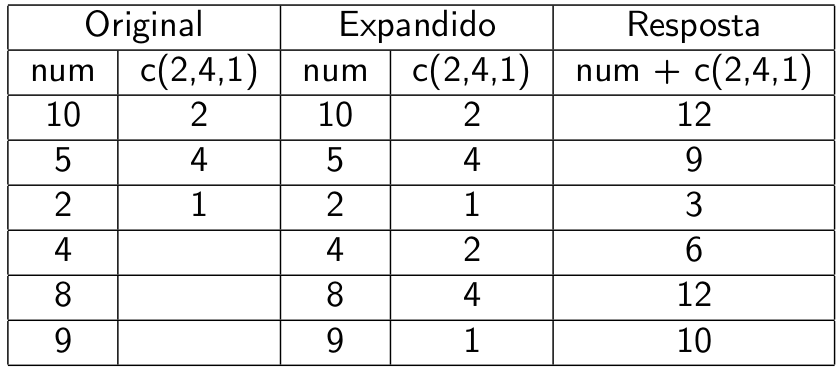
\includegraphics[width=0.8\linewidth]{img/reciclagem} \end{center}

Agora tente:

\begin{Shaded}
\begin{Highlighting}[]
\NormalTok{num }\OperatorTok{+}\StringTok{ }\KeywordTok{c}\NormalTok{(}\DecValTok{2}\NormalTok{, }\DecValTok{4}\NormalTok{, }\DecValTok{1}\NormalTok{, }\DecValTok{3}\NormalTok{)}
\end{Highlighting}
\end{Shaded}

\subsection{Outros tipos de vetores}\label{outros-tipos-de-vetores}

Vetores também podem ter outros tipos:

\begin{itemize}
\tightlist
\item
  Vetor de caracteres:
\end{itemize}

\begin{Shaded}
\begin{Highlighting}[]
\NormalTok{caracter <-}\StringTok{ }\KeywordTok{c}\NormalTok{(}\StringTok{"brava"}\NormalTok{, }\StringTok{"joaquina"}\NormalTok{, }\StringTok{"armação"}\NormalTok{)}
\NormalTok{caracter}
\NormalTok{[}\DecValTok{1}\NormalTok{] }\StringTok{"brava"}    \StringTok{"joaquina"} \StringTok{"armação"} 
\KeywordTok{typeof}\NormalTok{(caracter)}
\NormalTok{[}\DecValTok{1}\NormalTok{] }\StringTok{"character"}
\KeywordTok{class}\NormalTok{(caracter)}
\NormalTok{[}\DecValTok{1}\NormalTok{] }\StringTok{"character"}
\end{Highlighting}
\end{Shaded}

\begin{itemize}
\tightlist
\item
  Vetor lógico:
\end{itemize}

\begin{Shaded}
\begin{Highlighting}[]
\NormalTok{logico <-}\StringTok{ }\NormalTok{caracter }\OperatorTok{==}\StringTok{ "armação"}
\NormalTok{logico}
\NormalTok{[}\DecValTok{1}\NormalTok{] }\OtherTok{FALSE} \OtherTok{FALSE}  \OtherTok{TRUE}
\KeywordTok{typeof}\NormalTok{(logico)}
\NormalTok{[}\DecValTok{1}\NormalTok{] }\StringTok{"logical"}
\KeywordTok{class}\NormalTok{(logico)}
\NormalTok{[}\DecValTok{1}\NormalTok{] }\StringTok{"logical"}
\end{Highlighting}
\end{Shaded}

ou

\begin{Shaded}
\begin{Highlighting}[]
\NormalTok{logico <-}\StringTok{ }\NormalTok{num }\OperatorTok{>}\StringTok{ }\DecValTok{4}
\NormalTok{logico}
\NormalTok{[}\DecValTok{1}\NormalTok{]  }\OtherTok{TRUE}  \OtherTok{TRUE} \OtherTok{FALSE} \OtherTok{FALSE}  \OtherTok{TRUE}  \OtherTok{TRUE}
\end{Highlighting}
\end{Shaded}

No exemplo anterior, a condição \texttt{num\ \textgreater{}\ 4} é uma
\textbf{expressão condicional}, e o símbolo \texttt{\textgreater{}} um
\textbf{operador lógico}. Os operadores lógicos utilizados no R são:

\begin{longtable}[]{@{}cll@{}}
\toprule
Operador & Sintaxe & Teste\tabularnewline
\midrule
\endhead
\texttt{\textless{}} & \texttt{a\ \textless{}\ b} & \texttt{a} é menor
que \texttt{b}?\tabularnewline
\texttt{\textless{}=} & \texttt{a\ \textless{}=\ b} & \texttt{a} é menor
ou igual a \texttt{b}?\tabularnewline
\texttt{\textgreater{}} & \texttt{a\ \textgreater{}\ b} & \texttt{a} é
maior que \texttt{b}\tabularnewline
\texttt{\textgreater{}=} & \texttt{a\ \textgreater{}=\ b} & \texttt{a} é
maior ou igual a \texttt{b}?\tabularnewline
\texttt{==} & \texttt{a\ ==\ b} & \texttt{a} é igual a
\texttt{b}?\tabularnewline
\texttt{!=} & \texttt{a\ !=\ b} & \texttt{a} é diferente de
\texttt{b}?\tabularnewline
\texttt{\%in\%} & \texttt{a\ \%in\%\ c(a,\ b)} & \texttt{a} está contido
no vetor \texttt{c(a,\ b)}?\tabularnewline
\bottomrule
\end{longtable}

\subsection{Misturando classes de
objetos}\label{misturando-classes-de-objetos}

Algumas vezes isso acontece por acidente, mas também pode acontecer de
propósito.

O que acontece aqui?

\begin{Shaded}
\begin{Highlighting}[]
\NormalTok{w <-}\StringTok{ }\KeywordTok{c}\NormalTok{(5L, }\StringTok{"a"}\NormalTok{)}
\NormalTok{x <-}\StringTok{ }\KeywordTok{c}\NormalTok{(}\FloatTok{1.7}\NormalTok{, }\StringTok{"a"}\NormalTok{)}
\NormalTok{y <-}\StringTok{ }\KeywordTok{c}\NormalTok{(}\OtherTok{TRUE}\NormalTok{, }\DecValTok{2}\NormalTok{)}
\NormalTok{z <-}\StringTok{ }\KeywordTok{c}\NormalTok{(}\StringTok{"a"}\NormalTok{, T)}
\end{Highlighting}
\end{Shaded}

Lembre-se da regra:

Um vetor só pode conter elementos do mesmo tipo

Quando objetos de diferentes tipos são misturados, ocorre a
\textbf{coerção}, para que cada elemento possua a mesma classe.

Nos exemplos acima, nós vemos o efeito da \textbf{coerção implícita},
quando o R tenta representar todos os objetos de uma única forma.

Nós podemos forçar um objeto a mudar de classe, através da
\textbf{coerção explícita}, realizada pelas funções \texttt{as.*}:

\begin{Shaded}
\begin{Highlighting}[]
\NormalTok{x <-}\StringTok{ }\DecValTok{0}\OperatorTok{:}\DecValTok{6}
\KeywordTok{typeof}\NormalTok{(x)}
\NormalTok{[}\DecValTok{1}\NormalTok{] }\StringTok{"integer"}
\KeywordTok{class}\NormalTok{(x)}
\NormalTok{[}\DecValTok{1}\NormalTok{] }\StringTok{"integer"}
\KeywordTok{as.numeric}\NormalTok{(x)}
\NormalTok{[}\DecValTok{1}\NormalTok{] }\DecValTok{0} \DecValTok{1} \DecValTok{2} \DecValTok{3} \DecValTok{4} \DecValTok{5} \DecValTok{6}
\KeywordTok{as.logical}\NormalTok{(x)}
\NormalTok{[}\DecValTok{1}\NormalTok{] }\OtherTok{FALSE}  \OtherTok{TRUE}  \OtherTok{TRUE}  \OtherTok{TRUE}  \OtherTok{TRUE}  \OtherTok{TRUE}  \OtherTok{TRUE}
\KeywordTok{as.character}\NormalTok{(x)}
\NormalTok{[}\DecValTok{1}\NormalTok{] }\StringTok{"0"} \StringTok{"1"} \StringTok{"2"} \StringTok{"3"} \StringTok{"4"} \StringTok{"5"} \StringTok{"6"}
\KeywordTok{as.factor}\NormalTok{(x)}
\NormalTok{[}\DecValTok{1}\NormalTok{] }\DecValTok{0} \DecValTok{1} \DecValTok{2} \DecValTok{3} \DecValTok{4} \DecValTok{5} \DecValTok{6}
\NormalTok{Levels}\OperatorTok{:}\StringTok{ }\DecValTok{0} \DecValTok{1} \DecValTok{2} \DecValTok{3} \DecValTok{4} \DecValTok{5} \DecValTok{6}
\end{Highlighting}
\end{Shaded}

De \texttt{?logical}:

\begin{verbatim}
 Logical vectors are coerced to integer vectors in contexts where a
 numerical value is required, with ‘TRUE’ being mapped to ‘1L’,
 ‘FALSE’ to ‘0L’ and ‘NA’ to ‘NA_integer_’.
\end{verbatim}

\begin{Shaded}
\begin{Highlighting}[]
\NormalTok{(x <-}\StringTok{ }\KeywordTok{c}\NormalTok{(}\OtherTok{FALSE}\NormalTok{, }\OtherTok{TRUE}\NormalTok{))}
\NormalTok{[}\DecValTok{1}\NormalTok{] }\OtherTok{FALSE}  \OtherTok{TRUE}
\KeywordTok{class}\NormalTok{(x)}
\NormalTok{[}\DecValTok{1}\NormalTok{] }\StringTok{"logical"}
\KeywordTok{as.numeric}\NormalTok{(x)}
\NormalTok{[}\DecValTok{1}\NormalTok{] }\DecValTok{0} \DecValTok{1}
\end{Highlighting}
\end{Shaded}

Algumas vezes não é possível fazer a coerção, então:

\begin{Shaded}
\begin{Highlighting}[]
\NormalTok{x <-}\StringTok{ }\KeywordTok{c}\NormalTok{(}\StringTok{"a"}\NormalTok{, }\StringTok{"b"}\NormalTok{, }\StringTok{"c"}\NormalTok{)}
\KeywordTok{as.numeric}\NormalTok{(x)}
\NormalTok{Warning}\OperatorTok{:}\StringTok{ }\NormalTok{NAs introduced by coercion}
\NormalTok{[}\DecValTok{1}\NormalTok{] }\OtherTok{NA} \OtherTok{NA} \OtherTok{NA}
\KeywordTok{as.logical}\NormalTok{(x)}
\NormalTok{[}\DecValTok{1}\NormalTok{] }\OtherTok{NA} \OtherTok{NA} \OtherTok{NA}
\end{Highlighting}
\end{Shaded}

\subsection{Valores perdidos e
especiais}\label{valores-perdidos-e-especiais}

Valores perdidos devem ser definidos como \texttt{NA} (\emph{not
available}):

\begin{Shaded}
\begin{Highlighting}[]
\NormalTok{perd <-}\StringTok{ }\KeywordTok{c}\NormalTok{(}\DecValTok{3}\NormalTok{, }\DecValTok{5}\NormalTok{, }\OtherTok{NA}\NormalTok{, }\DecValTok{2}\NormalTok{)}
\NormalTok{perd}
\NormalTok{[}\DecValTok{1}\NormalTok{]  }\DecValTok{3}  \DecValTok{5} \OtherTok{NA}  \DecValTok{2}
\KeywordTok{class}\NormalTok{(perd)}
\NormalTok{[}\DecValTok{1}\NormalTok{] }\StringTok{"numeric"}
\end{Highlighting}
\end{Shaded}

Podemos testar a presença de \texttt{NA}s com a função \texttt{is.na()}:

\begin{Shaded}
\begin{Highlighting}[]
\KeywordTok{is.na}\NormalTok{(perd)}
\NormalTok{[}\DecValTok{1}\NormalTok{] }\OtherTok{FALSE} \OtherTok{FALSE}  \OtherTok{TRUE} \OtherTok{FALSE}
\end{Highlighting}
\end{Shaded}

Ou:

\begin{Shaded}
\begin{Highlighting}[]
\KeywordTok{any}\NormalTok{(}\KeywordTok{is.na}\NormalTok{(perd))}
\NormalTok{[}\DecValTok{1}\NormalTok{] }\OtherTok{TRUE}
\end{Highlighting}
\end{Shaded}

Outros valores especiais são:

\begin{itemize}
\tightlist
\item
  \texttt{NaN} (\emph{not a number}) - exemplo: \texttt{0/0}
\item
  \texttt{-Inf} e \texttt{Inf} - exemplo: \texttt{1/0}
\end{itemize}

A função \texttt{is.na()} também testa a presença de \texttt{NaN}s:

\begin{Shaded}
\begin{Highlighting}[]
\NormalTok{perd <-}\StringTok{ }\KeywordTok{c}\NormalTok{(}\OperatorTok{-}\DecValTok{1}\NormalTok{,}\DecValTok{0}\NormalTok{,}\DecValTok{1}\NormalTok{)}\OperatorTok{/}\DecValTok{0}
\NormalTok{perd}
\NormalTok{[}\DecValTok{1}\NormalTok{] }\OperatorTok{-}\OtherTok{Inf}  \OtherTok{NaN}  \OtherTok{Inf}
\KeywordTok{is.na}\NormalTok{(perd)}
\NormalTok{[}\DecValTok{1}\NormalTok{] }\OtherTok{FALSE}  \OtherTok{TRUE} \OtherTok{FALSE}
\end{Highlighting}
\end{Shaded}

A função \texttt{is.infinite()} testa se há valores infinitos

\begin{Shaded}
\begin{Highlighting}[]
\KeywordTok{is.infinite}\NormalTok{(perd)}
\NormalTok{[}\DecValTok{1}\NormalTok{]  }\OtherTok{TRUE} \OtherTok{FALSE}  \OtherTok{TRUE}
\end{Highlighting}
\end{Shaded}

\section*{Exercícios}\label{exercicios-3}


\begin{enumerate}
\def\labelenumi{\arabic{enumi}.}
\tightlist
\item
  Crie um objeto com os valores 54, 0, 17, 94, 12.5, 2, 0.9, 15.

  \begin{enumerate}
  \def\labelenumii{\alph{enumii}.}
  \tightlist
  \item
    Some o objeto acima com os valores 5, 6, e depois com os valores 5,
    6, 7.
  \end{enumerate}
\item
  Construa um único objeto com as letras: \texttt{A}, \texttt{B}, e
  \texttt{C}, repetidas cada uma 15, 12, e 8 vezes, respectivamente.

  \begin{enumerate}
  \def\labelenumii{\alph{enumii}.}
  \tightlist
  \item
    Mostre na tela, em forma de verdadeiro ou falso, onde estão as
    letras \texttt{B} nesse objeto.
  \item
    Veja a página de ajuda da função \texttt{sum()} e descubra como
    fazer para contar o número de letras \texttt{B} neste vetor (usando
    \texttt{sum()}).
  \end{enumerate}
\item
  Crie um objeto com 100 valores aleatórios de uma distribuição uniforme
  \(U(0,1)\). Conte quantas vezes aparecem valores maiores ou iguais a
  0,5.
\item
  Calcule as 50 primeiras potências de 2, ou seja,
  \(2, 2^2, 2^3,  \ldots, 2^{50}\).

  \begin{enumerate}
  \def\labelenumii{\alph{enumii}.}
  \tightlist
  \item
    Calcule o quadrado dos números inteiros de 1 a 50, ou seja,
    \(1^2, 2^2, 3^2, \ldots, 50^2\).
  \item
    Quais pares são iguais, ou seja, quais números inteiros dos dois
    exercícios anteriores satisfazem a condição \(2^n = n^2\)?
  \item
    Quantos pares existem?
  \end{enumerate}
\item
  Calcule o seno, coseno e a tangente para os números variando de \(0\)
  a \(2\pi\), com distância de \(0.1\) entre eles. (Use as funções
  \texttt{sin()}, \texttt{cos()}, \texttt{tan()}).

  \begin{enumerate}
  \def\labelenumii{\alph{enumii}.}
  \tightlist
  \item
    Calcule a tangente usando a relação \(\tan(x) = \sin(x)/\cos(x)\).
  \item
    Calcule as diferenças das tangentes calculadas pela função do R e
    pela razão acima.
  \item
    Quais valores são exatamente iguais?
  \item
    Qual a diferença máxima (em módulo) entre eles? Qual é a causa dessa
    diferença?
  \end{enumerate}
\end{enumerate}

\section{Outras classes}\label{outras-classes}

Como mencionado na seção anterior, o R possui 6 tipos básicos de
estrutura de dados, mas diversas classes podem ser construídas a partir
destes tipos básicos. Abaixo, veremos algumas das mais importantes.

\subsection{Fator}\label{fator}

Os fatores são parecidos com caracteres no R, mas são armazenados e
tratados de maneira diferente.

Características:

\begin{itemize}
\tightlist
\item
  Coleção de categorias ou \textbf{níveis} (\emph{levels})
\item
  Estrutura unidimensional
\end{itemize}

Utilizando as funções \texttt{factor()} e \texttt{c()}:

\begin{Shaded}
\begin{Highlighting}[]
\NormalTok{fator <-}\StringTok{ }\KeywordTok{factor}\NormalTok{(}\KeywordTok{c}\NormalTok{(}\StringTok{"alta"}\NormalTok{,}\StringTok{"baixa"}\NormalTok{,}\StringTok{"baixa"}\NormalTok{,}\StringTok{"media"}\NormalTok{,}
                  \StringTok{"alta"}\NormalTok{,}\StringTok{"media"}\NormalTok{,}\StringTok{"baixa"}\NormalTok{,}\StringTok{"media"}\NormalTok{,}\StringTok{"media"}\NormalTok{))}
\NormalTok{fator}
\NormalTok{[}\DecValTok{1}\NormalTok{] alta  baixa baixa media alta  media baixa media media}
\NormalTok{Levels}\OperatorTok{:}\StringTok{ }\NormalTok{alta baixa media}
\KeywordTok{class}\NormalTok{(fator)}
\NormalTok{[}\DecValTok{1}\NormalTok{] }\StringTok{"factor"}
\KeywordTok{typeof}\NormalTok{(fator)}
\NormalTok{[}\DecValTok{1}\NormalTok{] }\StringTok{"integer"}
\end{Highlighting}
\end{Shaded}

Note que o objeto é da classe \texttt{factor}, mas seu tipo básico é
\texttt{integer}! Isso significa que cada categoria única é identificada
internamente por um número, e isso faz com que os fatores possuam uma
ordenação, de acordo com as categorias únicas. Por isso existe a
identificação dos \texttt{Levels} (níveis) de um fator.

Veja o que acontece quando ``remover a classe'' desse objeto

\begin{Shaded}
\begin{Highlighting}[]
\KeywordTok{unclass}\NormalTok{(fator)}
\NormalTok{[}\DecValTok{1}\NormalTok{] }\DecValTok{1} \DecValTok{2} \DecValTok{2} \DecValTok{3} \DecValTok{1} \DecValTok{3} \DecValTok{2} \DecValTok{3} \DecValTok{3}
\KeywordTok{attr}\NormalTok{(,}\StringTok{"levels"}\NormalTok{)}
\NormalTok{[}\DecValTok{1}\NormalTok{] }\StringTok{"alta"}  \StringTok{"baixa"} \StringTok{"media"}
\end{Highlighting}
\end{Shaded}

Fatores podem ser convertidos para caracteres, e \textbf{também} para
números inteiros

\begin{Shaded}
\begin{Highlighting}[]
\KeywordTok{as.character}\NormalTok{(fator)}
\NormalTok{[}\DecValTok{1}\NormalTok{] }\StringTok{"alta"}  \StringTok{"baixa"} \StringTok{"baixa"} \StringTok{"media"} \StringTok{"alta"}  \StringTok{"media"} \StringTok{"baixa"} \StringTok{"media"} \StringTok{"media"}
\KeywordTok{as.integer}\NormalTok{(fator)}
\NormalTok{[}\DecValTok{1}\NormalTok{] }\DecValTok{1} \DecValTok{2} \DecValTok{2} \DecValTok{3} \DecValTok{1} \DecValTok{3} \DecValTok{2} \DecValTok{3} \DecValTok{3}
\end{Highlighting}
\end{Shaded}

Caso haja uma hierarquia, os níveis dos fatores podem ser ordenados
explicitamente através do argumento \texttt{levels}:

\begin{Shaded}
\begin{Highlighting}[]
\NormalTok{fator <-}\StringTok{ }\KeywordTok{factor}\NormalTok{(}\KeywordTok{c}\NormalTok{(}\StringTok{"alta"}\NormalTok{,}\StringTok{"baixa"}\NormalTok{,}\StringTok{"baixa"}\NormalTok{,}\StringTok{"media"}\NormalTok{,}
                  \StringTok{"alta"}\NormalTok{,}\StringTok{"media"}\NormalTok{,}\StringTok{"baixa"}\NormalTok{,}\StringTok{"media"}\NormalTok{,}\StringTok{"media"}\NormalTok{),}
                \DataTypeTok{levels =} \KeywordTok{c}\NormalTok{(}\StringTok{"alta"}\NormalTok{,}\StringTok{"media"}\NormalTok{,}\StringTok{"baixa"}\NormalTok{))}
\NormalTok{fator}
\NormalTok{[}\DecValTok{1}\NormalTok{] alta  baixa baixa media alta  media baixa media media}
\NormalTok{Levels}\OperatorTok{:}\StringTok{ }\NormalTok{alta media baixa}
\KeywordTok{typeof}\NormalTok{(fator)}
\NormalTok{[}\DecValTok{1}\NormalTok{] }\StringTok{"integer"}
\KeywordTok{class}\NormalTok{(fator)}
\NormalTok{[}\DecValTok{1}\NormalTok{] }\StringTok{"factor"}
\end{Highlighting}
\end{Shaded}

Além disso, os níveis dos fatores podem também ser explicitamente
ordenados

\begin{Shaded}
\begin{Highlighting}[]
\NormalTok{fator <-}\StringTok{ }\KeywordTok{factor}\NormalTok{(}\KeywordTok{c}\NormalTok{(}\StringTok{"alta"}\NormalTok{,}\StringTok{"baixa"}\NormalTok{,}\StringTok{"baixa"}\NormalTok{,}\StringTok{"media"}\NormalTok{,}
                  \StringTok{"alta"}\NormalTok{,}\StringTok{"media"}\NormalTok{,}\StringTok{"baixa"}\NormalTok{,}\StringTok{"media"}\NormalTok{,}\StringTok{"media"}\NormalTok{),}
                \DataTypeTok{levels =} \KeywordTok{c}\NormalTok{(}\StringTok{"baixa"}\NormalTok{, }\StringTok{"media"}\NormalTok{, }\StringTok{"alta"}\NormalTok{),}
                \DataTypeTok{ordered =} \OtherTok{TRUE}\NormalTok{)}
\NormalTok{fator}
\NormalTok{[}\DecValTok{1}\NormalTok{] alta  baixa baixa media alta  media baixa media media}
\NormalTok{Levels}\OperatorTok{:}\StringTok{ }\NormalTok{baixa }\OperatorTok{<}\StringTok{ }\NormalTok{media }\OperatorTok{<}\StringTok{ }\NormalTok{alta}
\KeywordTok{typeof}\NormalTok{(fator)}
\NormalTok{[}\DecValTok{1}\NormalTok{] }\StringTok{"integer"}
\KeywordTok{class}\NormalTok{(fator)}
\NormalTok{[}\DecValTok{1}\NormalTok{] }\StringTok{"ordered"} \StringTok{"factor"} 
\end{Highlighting}
\end{Shaded}

(Veja que um objeto pode ter mais de uma classe). Isso geralmente só
será útil em casos especificos.

As seguintes funções são úteis para verificar os níveis e o número de
níveis de um fator:

\begin{Shaded}
\begin{Highlighting}[]
\KeywordTok{levels}\NormalTok{(fator)}
\NormalTok{[}\DecValTok{1}\NormalTok{] }\StringTok{"baixa"} \StringTok{"media"} \StringTok{"alta"} 
\KeywordTok{nlevels}\NormalTok{(fator)}
\NormalTok{[}\DecValTok{1}\NormalTok{] }\DecValTok{3}
\end{Highlighting}
\end{Shaded}

\subsection{Matriz}\label{matriz}

Matrizes são vetores que podem ser dispostos em duas dimensões.

Características:

\begin{itemize}
\tightlist
\item
  Podem conter apenas um tipo de informação (números, caracteres)
\item
  Estrutura bidimensional
\end{itemize}

Utilizando a função \texttt{matrix()}:

\begin{Shaded}
\begin{Highlighting}[]
\NormalTok{matriz <-}\StringTok{ }\KeywordTok{matrix}\NormalTok{(}\DecValTok{1}\OperatorTok{:}\DecValTok{12}\NormalTok{, }\DataTypeTok{nrow =} \DecValTok{3}\NormalTok{, }\DataTypeTok{ncol =} \DecValTok{4}\NormalTok{)}
\NormalTok{matriz}
\NormalTok{     [,}\DecValTok{1}\NormalTok{] [,}\DecValTok{2}\NormalTok{] [,}\DecValTok{3}\NormalTok{] [,}\DecValTok{4}\NormalTok{]}
\NormalTok{[}\DecValTok{1}\NormalTok{,]    }\DecValTok{1}    \DecValTok{4}    \DecValTok{7}   \DecValTok{10}
\NormalTok{[}\DecValTok{2}\NormalTok{,]    }\DecValTok{2}    \DecValTok{5}    \DecValTok{8}   \DecValTok{11}
\NormalTok{[}\DecValTok{3}\NormalTok{,]    }\DecValTok{3}    \DecValTok{6}    \DecValTok{9}   \DecValTok{12}
\KeywordTok{class}\NormalTok{(matriz)}
\NormalTok{[}\DecValTok{1}\NormalTok{] }\StringTok{"matrix"}
\KeywordTok{typeof}\NormalTok{(matriz)}
\NormalTok{[}\DecValTok{1}\NormalTok{] }\StringTok{"integer"}
\end{Highlighting}
\end{Shaded}

Alterando a ordem de preenchimento da matriz (por linhas):

\begin{Shaded}
\begin{Highlighting}[]
\NormalTok{matriz <-}\StringTok{ }\KeywordTok{matrix}\NormalTok{(}\DecValTok{1}\OperatorTok{:}\DecValTok{12}\NormalTok{, }\DataTypeTok{nrow =} \DecValTok{3}\NormalTok{, }\DataTypeTok{ncol =} \DecValTok{4}\NormalTok{, }\DataTypeTok{byrow =} \OtherTok{TRUE}\NormalTok{)}
\NormalTok{matriz}
\NormalTok{     [,}\DecValTok{1}\NormalTok{] [,}\DecValTok{2}\NormalTok{] [,}\DecValTok{3}\NormalTok{] [,}\DecValTok{4}\NormalTok{]}
\NormalTok{[}\DecValTok{1}\NormalTok{,]    }\DecValTok{1}    \DecValTok{2}    \DecValTok{3}    \DecValTok{4}
\NormalTok{[}\DecValTok{2}\NormalTok{,]    }\DecValTok{5}    \DecValTok{6}    \DecValTok{7}    \DecValTok{8}
\NormalTok{[}\DecValTok{3}\NormalTok{,]    }\DecValTok{9}   \DecValTok{10}   \DecValTok{11}   \DecValTok{12}
\end{Highlighting}
\end{Shaded}

Para verificar a dimensão da matriz:

\begin{Shaded}
\begin{Highlighting}[]
\KeywordTok{dim}\NormalTok{(matriz)}
\NormalTok{[}\DecValTok{1}\NormalTok{] }\DecValTok{3} \DecValTok{4}
\end{Highlighting}
\end{Shaded}

Adicionando colunas com \texttt{cbind()}

\begin{Shaded}
\begin{Highlighting}[]
\KeywordTok{cbind}\NormalTok{(matriz, }\KeywordTok{rep}\NormalTok{(}\DecValTok{99}\NormalTok{, }\DecValTok{3}\NormalTok{))}
\NormalTok{     [,}\DecValTok{1}\NormalTok{] [,}\DecValTok{2}\NormalTok{] [,}\DecValTok{3}\NormalTok{] [,}\DecValTok{4}\NormalTok{] [,}\DecValTok{5}\NormalTok{]}
\NormalTok{[}\DecValTok{1}\NormalTok{,]    }\DecValTok{1}    \DecValTok{2}    \DecValTok{3}    \DecValTok{4}   \DecValTok{99}
\NormalTok{[}\DecValTok{2}\NormalTok{,]    }\DecValTok{5}    \DecValTok{6}    \DecValTok{7}    \DecValTok{8}   \DecValTok{99}
\NormalTok{[}\DecValTok{3}\NormalTok{,]    }\DecValTok{9}   \DecValTok{10}   \DecValTok{11}   \DecValTok{12}   \DecValTok{99}
\end{Highlighting}
\end{Shaded}

Adicionando linhas com \texttt{rbind()}

\begin{Shaded}
\begin{Highlighting}[]
\KeywordTok{rbind}\NormalTok{(matriz, }\KeywordTok{rep}\NormalTok{(}\DecValTok{99}\NormalTok{, }\DecValTok{4}\NormalTok{))}
\NormalTok{     [,}\DecValTok{1}\NormalTok{] [,}\DecValTok{2}\NormalTok{] [,}\DecValTok{3}\NormalTok{] [,}\DecValTok{4}\NormalTok{]}
\NormalTok{[}\DecValTok{1}\NormalTok{,]    }\DecValTok{1}    \DecValTok{2}    \DecValTok{3}    \DecValTok{4}
\NormalTok{[}\DecValTok{2}\NormalTok{,]    }\DecValTok{5}    \DecValTok{6}    \DecValTok{7}    \DecValTok{8}
\NormalTok{[}\DecValTok{3}\NormalTok{,]    }\DecValTok{9}   \DecValTok{10}   \DecValTok{11}   \DecValTok{12}
\NormalTok{[}\DecValTok{4}\NormalTok{,]   }\DecValTok{99}   \DecValTok{99}   \DecValTok{99}   \DecValTok{99}
\end{Highlighting}
\end{Shaded}

Matrizes também podem ser criadas a partir de vetores adicionando um
\textbf{atributo} de dimensão

\begin{Shaded}
\begin{Highlighting}[]
\NormalTok{m <-}\StringTok{ }\DecValTok{1}\OperatorTok{:}\DecValTok{10}
\NormalTok{m}
\NormalTok{ [}\DecValTok{1}\NormalTok{]  }\DecValTok{1}  \DecValTok{2}  \DecValTok{3}  \DecValTok{4}  \DecValTok{5}  \DecValTok{6}  \DecValTok{7}  \DecValTok{8}  \DecValTok{9} \DecValTok{10}
\KeywordTok{class}\NormalTok{(m)}
\NormalTok{[}\DecValTok{1}\NormalTok{] }\StringTok{"integer"}
\KeywordTok{dim}\NormalTok{(m)}
\OtherTok{NULL}
\KeywordTok{dim}\NormalTok{(m) <-}\StringTok{ }\KeywordTok{c}\NormalTok{(}\DecValTok{2}\NormalTok{, }\DecValTok{5}\NormalTok{)}
\NormalTok{m}
\NormalTok{     [,}\DecValTok{1}\NormalTok{] [,}\DecValTok{2}\NormalTok{] [,}\DecValTok{3}\NormalTok{] [,}\DecValTok{4}\NormalTok{] [,}\DecValTok{5}\NormalTok{]}
\NormalTok{[}\DecValTok{1}\NormalTok{,]    }\DecValTok{1}    \DecValTok{3}    \DecValTok{5}    \DecValTok{7}    \DecValTok{9}
\NormalTok{[}\DecValTok{2}\NormalTok{,]    }\DecValTok{2}    \DecValTok{4}    \DecValTok{6}    \DecValTok{8}   \DecValTok{10}
\KeywordTok{class}\NormalTok{(m)}
\NormalTok{[}\DecValTok{1}\NormalTok{] }\StringTok{"matrix"}
\KeywordTok{typeof}\NormalTok{(m)}
\NormalTok{[}\DecValTok{1}\NormalTok{] }\StringTok{"integer"}
\end{Highlighting}
\end{Shaded}

\subsubsection{Operações matemáticas em
matrizes}\label{operacoes-matematicas-em-matrizes}

Matriz multiplicada por um escalar

\begin{Shaded}
\begin{Highlighting}[]
\NormalTok{matriz }\OperatorTok{*}\StringTok{ }\DecValTok{2}
\NormalTok{     [,}\DecValTok{1}\NormalTok{] [,}\DecValTok{2}\NormalTok{] [,}\DecValTok{3}\NormalTok{] [,}\DecValTok{4}\NormalTok{]}
\NormalTok{[}\DecValTok{1}\NormalTok{,]    }\DecValTok{2}    \DecValTok{4}    \DecValTok{6}    \DecValTok{8}
\NormalTok{[}\DecValTok{2}\NormalTok{,]   }\DecValTok{10}   \DecValTok{12}   \DecValTok{14}   \DecValTok{16}
\NormalTok{[}\DecValTok{3}\NormalTok{,]   }\DecValTok{18}   \DecValTok{20}   \DecValTok{22}   \DecValTok{24}
\end{Highlighting}
\end{Shaded}

Multiplicação de matrizes (observe as dimensões!)

\begin{Shaded}
\begin{Highlighting}[]
\NormalTok{matriz2 <-}\StringTok{ }\KeywordTok{matrix}\NormalTok{(}\DecValTok{1}\NormalTok{, }\DataTypeTok{nrow =} \DecValTok{4}\NormalTok{, }\DataTypeTok{ncol =} \DecValTok{3}\NormalTok{)}
\NormalTok{matriz }\OperatorTok\StringTok{ }\NormalTok{matriz2}
\NormalTok{     [,}\DecValTok{1}\NormalTok{] [,}\DecValTok{2}\NormalTok{] [,}\DecValTok{3}\NormalTok{]}
\NormalTok{[}\DecValTok{1}\NormalTok{,]   }\DecValTok{10}   \DecValTok{10}   \DecValTok{10}
\NormalTok{[}\DecValTok{2}\NormalTok{,]   }\DecValTok{26}   \DecValTok{26}   \DecValTok{26}
\NormalTok{[}\DecValTok{3}\NormalTok{,]   }\DecValTok{42}   \DecValTok{42}   \DecValTok{42}
\end{Highlighting}
\end{Shaded}

\subsection{Array}\label{array}

Um array é a forma mais geral de uma matriz, pois pode ter \(n\)
dimensões.

Características:

\begin{itemize}
\tightlist
\item
  Estrutura \(n\)-dimensional
\item
  Assim como as matrizes, podem conter apenas um tipo de informação
  (números, caracteres)
\end{itemize}

Para criar um array, usamos a função \texttt{array()}, passando como
primeiro argumento um vetor atômico, e especificamos a dimensão com o
argumento \texttt{dim}. Por exemplo, para criar um objeto com 3
dimensões \(2 \times 2 \times 3\), fazemos

\begin{Shaded}
\begin{Highlighting}[]
\NormalTok{ar <-}\StringTok{ }\KeywordTok{array}\NormalTok{(}\DecValTok{1}\OperatorTok{:}\DecValTok{12}\NormalTok{, }\DataTypeTok{dim =} \KeywordTok{c}\NormalTok{(}\DecValTok{2}\NormalTok{, }\DecValTok{2}\NormalTok{, }\DecValTok{3}\NormalTok{))}
\NormalTok{ar}
\NormalTok{, , }\DecValTok{1}

\NormalTok{     [,}\DecValTok{1}\NormalTok{] [,}\DecValTok{2}\NormalTok{]}
\NormalTok{[}\DecValTok{1}\NormalTok{,]    }\DecValTok{1}    \DecValTok{3}
\NormalTok{[}\DecValTok{2}\NormalTok{,]    }\DecValTok{2}    \DecValTok{4}

\NormalTok{, , }\DecValTok{2}

\NormalTok{     [,}\DecValTok{1}\NormalTok{] [,}\DecValTok{2}\NormalTok{]}
\NormalTok{[}\DecValTok{1}\NormalTok{,]    }\DecValTok{5}    \DecValTok{7}
\NormalTok{[}\DecValTok{2}\NormalTok{,]    }\DecValTok{6}    \DecValTok{8}

\NormalTok{, , }\DecValTok{3}

\NormalTok{     [,}\DecValTok{1}\NormalTok{] [,}\DecValTok{2}\NormalTok{]}
\NormalTok{[}\DecValTok{1}\NormalTok{,]    }\DecValTok{9}   \DecValTok{11}
\NormalTok{[}\DecValTok{2}\NormalTok{,]   }\DecValTok{10}   \DecValTok{12}
\end{Highlighting}
\end{Shaded}

Similarmente, um array de 2 dimensões \(3 \times 2 \times 2\) é obtido
com

\begin{Shaded}
\begin{Highlighting}[]
\NormalTok{ar <-}\StringTok{ }\KeywordTok{array}\NormalTok{(}\DecValTok{1}\OperatorTok{:}\DecValTok{12}\NormalTok{, }\DataTypeTok{dim =} \KeywordTok{c}\NormalTok{(}\DecValTok{3}\NormalTok{, }\DecValTok{2}\NormalTok{, }\DecValTok{2}\NormalTok{))}
\NormalTok{ar}
\NormalTok{, , }\DecValTok{1}

\NormalTok{     [,}\DecValTok{1}\NormalTok{] [,}\DecValTok{2}\NormalTok{]}
\NormalTok{[}\DecValTok{1}\NormalTok{,]    }\DecValTok{1}    \DecValTok{4}
\NormalTok{[}\DecValTok{2}\NormalTok{,]    }\DecValTok{2}    \DecValTok{5}
\NormalTok{[}\DecValTok{3}\NormalTok{,]    }\DecValTok{3}    \DecValTok{6}

\NormalTok{, , }\DecValTok{2}

\NormalTok{     [,}\DecValTok{1}\NormalTok{] [,}\DecValTok{2}\NormalTok{]}
\NormalTok{[}\DecValTok{1}\NormalTok{,]    }\DecValTok{7}   \DecValTok{10}
\NormalTok{[}\DecValTok{2}\NormalTok{,]    }\DecValTok{8}   \DecValTok{11}
\NormalTok{[}\DecValTok{3}\NormalTok{,]    }\DecValTok{9}   \DecValTok{12}
\end{Highlighting}
\end{Shaded}

\subsection{Lista}\label{lista}

Como já vimos, uma lista não é uma ``classe'' propriamente dita, mas sim
um tipo de estrutura de dados básico, ao lado dos vetores atômicos. E,
assim como os vetores atômicos, listas são estruturas unidimensionais. A
grande diferença é que listas agrupam objetos de diferentes tipos,
inclusive outras listas.

Características:

\begin{itemize}
\tightlist
\item
  Pode combinar uma coleção de objetos de diferentes tipos ou classes (é
  um tipo básico de vetor, assim como os vetores atômicos)
\item
  Estrutura ``unidimensional'': apenas o número de elementos na lista é
  contado
\end{itemize}

Ppor exemplo, podemos criar uma lista com uma sequência de números, um
caracter e outra lista

\begin{Shaded}
\begin{Highlighting}[]
\NormalTok{lista <-}\StringTok{ }\KeywordTok{list}\NormalTok{(}\DecValTok{1}\OperatorTok{:}\DecValTok{30}\NormalTok{, }\StringTok{"R"}\NormalTok{, }\KeywordTok{list}\NormalTok{(}\OtherTok{TRUE}\NormalTok{, }\OtherTok{FALSE}\NormalTok{))}
\NormalTok{lista}
\NormalTok{[[}\DecValTok{1}\NormalTok{]]}
\NormalTok{ [}\DecValTok{1}\NormalTok{]  }\DecValTok{1}  \DecValTok{2}  \DecValTok{3}  \DecValTok{4}  \DecValTok{5}  \DecValTok{6}  \DecValTok{7}  \DecValTok{8}  \DecValTok{9} \DecValTok{10} \DecValTok{11} \DecValTok{12} \DecValTok{13} \DecValTok{14} \DecValTok{15} \DecValTok{16} \DecValTok{17} \DecValTok{18} \DecValTok{19} \DecValTok{20} \DecValTok{21} \DecValTok{22} \DecValTok{23}
\NormalTok{[}\DecValTok{24}\NormalTok{] }\DecValTok{24} \DecValTok{25} \DecValTok{26} \DecValTok{27} \DecValTok{28} \DecValTok{29} \DecValTok{30}

\NormalTok{[[}\DecValTok{2}\NormalTok{]]}
\NormalTok{[}\DecValTok{1}\NormalTok{] }\StringTok{"R"}

\NormalTok{[[}\DecValTok{3}\NormalTok{]]}
\NormalTok{[[}\DecValTok{3}\NormalTok{]][[}\DecValTok{1}\NormalTok{]]}
\NormalTok{[}\DecValTok{1}\NormalTok{] }\OtherTok{TRUE}

\NormalTok{[[}\DecValTok{3}\NormalTok{]][[}\DecValTok{2}\NormalTok{]]}
\NormalTok{[}\DecValTok{1}\NormalTok{] }\OtherTok{FALSE}
\KeywordTok{class}\NormalTok{(lista)}
\NormalTok{[}\DecValTok{1}\NormalTok{] }\StringTok{"list"}
\KeywordTok{typeof}\NormalTok{(lista)}
\NormalTok{[}\DecValTok{1}\NormalTok{] }\StringTok{"list"}
\end{Highlighting}
\end{Shaded}

Para melhor visualizar a estrutura dessa lista (ou de qualquer outro
objeto) poddemos usar a função \texttt{str()}

\begin{Shaded}
\begin{Highlighting}[]
\KeywordTok{str}\NormalTok{(lista)}
\NormalTok{List of }\DecValTok{3}
 \OperatorTok{$}\StringTok{ }\ErrorTok{:}\StringTok{ }\NormalTok{int [}\DecValTok{1}\OperatorTok{:}\DecValTok{30}\NormalTok{] }\DecValTok{1} \DecValTok{2} \DecValTok{3} \DecValTok{4} \DecValTok{5} \DecValTok{6} \DecValTok{7} \DecValTok{8} \DecValTok{9} \DecValTok{10}\NormalTok{ ...}
 \OperatorTok{$}\StringTok{ }\ErrorTok{:}\StringTok{ }\NormalTok{chr }\StringTok{"R"}
 \OperatorTok{$}\StringTok{ }\ErrorTok{:}\NormalTok{List of }\DecValTok{2}
\NormalTok{  ..}\OperatorTok{$}\StringTok{ }\ErrorTok{:}\StringTok{ }\NormalTok{logi }\OtherTok{TRUE}
\NormalTok{  ..}\OperatorTok{$}\StringTok{ }\ErrorTok{:}\StringTok{ }\NormalTok{logi }\OtherTok{FALSE}
\end{Highlighting}
\end{Shaded}

Note que de fato é uma estrutura unidimensional

\begin{Shaded}
\begin{Highlighting}[]
\KeywordTok{dim}\NormalTok{(lista)}
\OtherTok{NULL}
\KeywordTok{length}\NormalTok{(lista)}
\NormalTok{[}\DecValTok{1}\NormalTok{] }\DecValTok{3}
\end{Highlighting}
\end{Shaded}

Listas podem armazenar objetos de diferentes classes e dimensões, por
exemplo, usando objetos criados anteriormente

\begin{Shaded}
\begin{Highlighting}[]
\NormalTok{lista <-}\StringTok{ }\KeywordTok{list}\NormalTok{(fator, matriz)}
\NormalTok{lista}
\NormalTok{[[}\DecValTok{1}\NormalTok{]]}
\NormalTok{[}\DecValTok{1}\NormalTok{] alta  baixa baixa media alta  media baixa media media}
\NormalTok{Levels}\OperatorTok{:}\StringTok{ }\NormalTok{baixa }\OperatorTok{<}\StringTok{ }\NormalTok{media }\OperatorTok{<}\StringTok{ }\NormalTok{alta}

\NormalTok{[[}\DecValTok{2}\NormalTok{]]}
\NormalTok{     [,}\DecValTok{1}\NormalTok{] [,}\DecValTok{2}\NormalTok{] [,}\DecValTok{3}\NormalTok{] [,}\DecValTok{4}\NormalTok{]}
\NormalTok{[}\DecValTok{1}\NormalTok{,]    }\DecValTok{1}    \DecValTok{2}    \DecValTok{3}    \DecValTok{4}
\NormalTok{[}\DecValTok{2}\NormalTok{,]    }\DecValTok{5}    \DecValTok{6}    \DecValTok{7}    \DecValTok{8}
\NormalTok{[}\DecValTok{3}\NormalTok{,]    }\DecValTok{9}   \DecValTok{10}   \DecValTok{11}   \DecValTok{12}
\KeywordTok{length}\NormalTok{(lista)}
\NormalTok{[}\DecValTok{1}\NormalTok{] }\DecValTok{2}
\end{Highlighting}
\end{Shaded}

\subsection{Data frame}\label{data-frame}

Data frame é a versão bidimensional de uma lista. Data frames
\textbf{são} listas, mas onde cada componente dever ter obrigatoriamente
o mesmo comprimento. Cada vetor da lista vira uma coluna em um data
frame, permitindo então que as ``colunas'' sejam de diferentes tipos.

Os data frames são as estruturas mais comuns para se trabalhar com dados
no R.

Características:

\begin{itemize}
\tightlist
\item
  Uma lista de vetores e/ou fatores, de \textbf{mesmo comprimento}
\item
  Pode conter diferentes tipos de dados (numérico, fator, \ldots{})
\item
  Estrutura bidimensional
\end{itemize}

Utilizando a função \texttt{data.frame()}:

\begin{Shaded}
\begin{Highlighting}[]
\NormalTok{da <-}\StringTok{ }\KeywordTok{data.frame}\NormalTok{(}\DataTypeTok{nome =} \KeywordTok{c}\NormalTok{(}\StringTok{"João"}\NormalTok{, }\StringTok{"José"}\NormalTok{, }\StringTok{"Maria"}\NormalTok{),}
                 \DataTypeTok{sexo =} \KeywordTok{c}\NormalTok{(}\StringTok{"M"}\NormalTok{, }\StringTok{"M"}\NormalTok{, }\StringTok{"F"}\NormalTok{),}
                 \DataTypeTok{idade =} \KeywordTok{c}\NormalTok{(}\DecValTok{32}\NormalTok{, }\DecValTok{34}\NormalTok{, }\DecValTok{30}\NormalTok{))}
\NormalTok{da}
\NormalTok{   nome sexo idade}
\DecValTok{1}\NormalTok{  João    M    }\DecValTok{32}
\DecValTok{2}\NormalTok{  José    M    }\DecValTok{34}
\DecValTok{3}\NormalTok{ Maria    F    }\DecValTok{30}
\KeywordTok{class}\NormalTok{(da)}
\NormalTok{[}\DecValTok{1}\NormalTok{] }\StringTok{"data.frame"}
\KeywordTok{typeof}\NormalTok{(da)}
\NormalTok{[}\DecValTok{1}\NormalTok{] }\StringTok{"list"}
\KeywordTok{dim}\NormalTok{(da)}
\NormalTok{[}\DecValTok{1}\NormalTok{] }\DecValTok{3} \DecValTok{3}
\end{Highlighting}
\end{Shaded}

Veja os detalhes com \texttt{str()}

\begin{Shaded}
\begin{Highlighting}[]
\KeywordTok{str}\NormalTok{(da)}
\StringTok{'data.frame'}\OperatorTok{:}\StringTok{   }\DecValTok{3}\NormalTok{ obs. of  }\DecValTok{3}\NormalTok{ variables}\OperatorTok{:}
\StringTok{ }\ErrorTok{$}\StringTok{ }\NormalTok{nome }\OperatorTok{:}\StringTok{ }\NormalTok{Factor w}\OperatorTok{/}\StringTok{ }\DecValTok{3}\NormalTok{ levels }\StringTok{"João"}\NormalTok{,}\StringTok{"José"}\NormalTok{,..}\OperatorTok{:}\StringTok{ }\DecValTok{1} \DecValTok{2} \DecValTok{3}
 \OperatorTok{$}\StringTok{ }\NormalTok{sexo }\OperatorTok{:}\StringTok{ }\NormalTok{Factor w}\OperatorTok{/}\StringTok{ }\DecValTok{2}\NormalTok{ levels }\StringTok{"F"}\NormalTok{,}\StringTok{"M"}\OperatorTok{:}\StringTok{ }\DecValTok{2} \DecValTok{2} \DecValTok{1}
 \OperatorTok{$}\StringTok{ }\NormalTok{idade}\OperatorTok{:}\StringTok{ }\NormalTok{num  }\DecValTok{32} \DecValTok{34} \DecValTok{30}
\end{Highlighting}
\end{Shaded}

Note que a função \texttt{data.frame()} converte caracteres para fator
automaticamente. Para que isso não aconteça, use o argumento
\texttt{stringsAsFactors\ =\ FALSE}

\begin{Shaded}
\begin{Highlighting}[]
\NormalTok{da <-}\StringTok{ }\KeywordTok{data.frame}\NormalTok{(}\DataTypeTok{nome =} \KeywordTok{c}\NormalTok{(}\StringTok{"João"}\NormalTok{, }\StringTok{"José"}\NormalTok{, }\StringTok{"Maria"}\NormalTok{),}
                 \DataTypeTok{sexo =} \KeywordTok{c}\NormalTok{(}\StringTok{"M"}\NormalTok{, }\StringTok{"M"}\NormalTok{, }\StringTok{"F"}\NormalTok{),}
                 \DataTypeTok{idade =} \KeywordTok{c}\NormalTok{(}\DecValTok{32}\NormalTok{, }\DecValTok{34}\NormalTok{, }\DecValTok{30}\NormalTok{),}
                 \DataTypeTok{stringsAsFactors =} \OtherTok{FALSE}\NormalTok{)}
\NormalTok{da}
\NormalTok{   nome sexo idade}
\DecValTok{1}\NormalTok{  João    M    }\DecValTok{32}
\DecValTok{2}\NormalTok{  José    M    }\DecValTok{34}
\DecValTok{3}\NormalTok{ Maria    F    }\DecValTok{30}
\KeywordTok{str}\NormalTok{(da)}
\StringTok{'data.frame'}\OperatorTok{:}\StringTok{   }\DecValTok{3}\NormalTok{ obs. of  }\DecValTok{3}\NormalTok{ variables}\OperatorTok{:}
\StringTok{ }\ErrorTok{$}\StringTok{ }\NormalTok{nome }\OperatorTok{:}\StringTok{ }\NormalTok{chr  }\StringTok{"João"} \StringTok{"José"} \StringTok{"Maria"}
 \OperatorTok{$}\StringTok{ }\NormalTok{sexo }\OperatorTok{:}\StringTok{ }\NormalTok{chr  }\StringTok{"M"} \StringTok{"M"} \StringTok{"F"}
 \OperatorTok{$}\StringTok{ }\NormalTok{idade}\OperatorTok{:}\StringTok{ }\NormalTok{num  }\DecValTok{32} \DecValTok{34} \DecValTok{30}
\end{Highlighting}
\end{Shaded}

Data frames podem ser formados com objetos criados anteriormente, desde
que tenham o mesmo comprimento:

\begin{Shaded}
\begin{Highlighting}[]
\KeywordTok{length}\NormalTok{(num)}
\NormalTok{[}\DecValTok{1}\NormalTok{] }\DecValTok{6}
\KeywordTok{length}\NormalTok{(fator)}
\NormalTok{[}\DecValTok{1}\NormalTok{] }\DecValTok{9}
\NormalTok{db <-}\StringTok{ }\KeywordTok{data.frame}\NormalTok{(}\DataTypeTok{numerico =} \KeywordTok{c}\NormalTok{(num, }\OtherTok{NA}\NormalTok{, }\OtherTok{NA}\NormalTok{, }\OtherTok{NA}\NormalTok{),}
                 \DataTypeTok{fator =}\NormalTok{ fator)}
\NormalTok{db}
\NormalTok{  numerico fator}
\DecValTok{1}       \DecValTok{10}\NormalTok{  alta}
\DecValTok{2}        \DecValTok{5}\NormalTok{ baixa}
\DecValTok{3}        \DecValTok{2}\NormalTok{ baixa}
\DecValTok{4}        \DecValTok{4}\NormalTok{ media}
\DecValTok{5}        \DecValTok{8}\NormalTok{  alta}
\DecValTok{6}        \DecValTok{9}\NormalTok{ media}
\DecValTok{7}       \OtherTok{NA}\NormalTok{ baixa}
\DecValTok{8}       \OtherTok{NA}\NormalTok{ media}
\DecValTok{9}       \OtherTok{NA}\NormalTok{ media}
\KeywordTok{str}\NormalTok{(db)}
\StringTok{'data.frame'}\OperatorTok{:}\StringTok{   }\DecValTok{9}\NormalTok{ obs. of  }\DecValTok{2}\NormalTok{ variables}\OperatorTok{:}
\StringTok{ }\ErrorTok{$}\StringTok{ }\NormalTok{numerico}\OperatorTok{:}\StringTok{ }\NormalTok{num  }\DecValTok{10} \DecValTok{5} \DecValTok{2} \DecValTok{4} \DecValTok{8} \DecValTok{9} \OtherTok{NA} \OtherTok{NA} \OtherTok{NA}
 \OperatorTok{$}\StringTok{ }\NormalTok{fator   }\OperatorTok{:}\StringTok{ }\NormalTok{Ord.factor w}\OperatorTok{/}\StringTok{ }\DecValTok{3}\NormalTok{ levels }\StringTok{"baixa"}\OperatorTok{<}\StringTok{"media"}\OperatorTok{<}\NormalTok{..}\OperatorTok{:}\StringTok{ }\DecValTok{3} \DecValTok{1} \DecValTok{1} \DecValTok{2} \DecValTok{3} \DecValTok{2} \DecValTok{1} \DecValTok{2} \DecValTok{2}
\end{Highlighting}
\end{Shaded}

Algumas vezes pode ser necessário converter um data frame para uma
matriz. Existem duas opções:

\begin{Shaded}
\begin{Highlighting}[]
\KeywordTok{as.matrix}\NormalTok{(db)}
\NormalTok{      numerico fator  }
\NormalTok{ [}\DecValTok{1}\NormalTok{,] }\StringTok{"10"}     \StringTok{"alta"} 
\NormalTok{ [}\DecValTok{2}\NormalTok{,] }\StringTok{" 5"}     \StringTok{"baixa"}
\NormalTok{ [}\DecValTok{3}\NormalTok{,] }\StringTok{" 2"}     \StringTok{"baixa"}
\NormalTok{ [}\DecValTok{4}\NormalTok{,] }\StringTok{" 4"}     \StringTok{"media"}
\NormalTok{ [}\DecValTok{5}\NormalTok{,] }\StringTok{" 8"}     \StringTok{"alta"} 
\NormalTok{ [}\DecValTok{6}\NormalTok{,] }\StringTok{" 9"}     \StringTok{"media"}
\NormalTok{ [}\DecValTok{7}\NormalTok{,] }\OtherTok{NA}       \StringTok{"baixa"}
\NormalTok{ [}\DecValTok{8}\NormalTok{,] }\OtherTok{NA}       \StringTok{"media"}
\NormalTok{ [}\DecValTok{9}\NormalTok{,] }\OtherTok{NA}       \StringTok{"media"}
\KeywordTok{data.matrix}\NormalTok{(db)}
\NormalTok{      numerico fator}
\NormalTok{ [}\DecValTok{1}\NormalTok{,]       }\DecValTok{10}     \DecValTok{3}
\NormalTok{ [}\DecValTok{2}\NormalTok{,]        }\DecValTok{5}     \DecValTok{1}
\NormalTok{ [}\DecValTok{3}\NormalTok{,]        }\DecValTok{2}     \DecValTok{1}
\NormalTok{ [}\DecValTok{4}\NormalTok{,]        }\DecValTok{4}     \DecValTok{2}
\NormalTok{ [}\DecValTok{5}\NormalTok{,]        }\DecValTok{8}     \DecValTok{3}
\NormalTok{ [}\DecValTok{6}\NormalTok{,]        }\DecValTok{9}     \DecValTok{2}
\NormalTok{ [}\DecValTok{7}\NormalTok{,]       }\OtherTok{NA}     \DecValTok{1}
\NormalTok{ [}\DecValTok{8}\NormalTok{,]       }\OtherTok{NA}     \DecValTok{2}
\NormalTok{ [}\DecValTok{9}\NormalTok{,]       }\OtherTok{NA}     \DecValTok{2}
\end{Highlighting}
\end{Shaded}

Geralmente é o resultado de \texttt{data.matrix()} o que você está
procurando.

Lembre que os níveis de um fator são armazenados internamente como
números: \(1^\circ\) nível = 1, \(2^\circ\) nível = 2, \(\ldots\)

\begin{Shaded}
\begin{Highlighting}[]
\NormalTok{fator}
\NormalTok{[}\DecValTok{1}\NormalTok{] alta  baixa baixa media alta  media baixa media media}
\NormalTok{Levels}\OperatorTok{:}\StringTok{ }\NormalTok{baixa }\OperatorTok{<}\StringTok{ }\NormalTok{media }\OperatorTok{<}\StringTok{ }\NormalTok{alta}
\KeywordTok{str}\NormalTok{(fator)}
\NormalTok{ Ord.factor w}\OperatorTok{/}\StringTok{ }\DecValTok{3}\NormalTok{ levels }\StringTok{"baixa"}\OperatorTok{<}\StringTok{"media"}\OperatorTok{<}\NormalTok{..}\OperatorTok{:}\StringTok{ }\DecValTok{3} \DecValTok{1} \DecValTok{1} \DecValTok{2} \DecValTok{3} \DecValTok{2} \DecValTok{1} \DecValTok{2} \DecValTok{2}
\KeywordTok{as.numeric}\NormalTok{(fator)}
\NormalTok{[}\DecValTok{1}\NormalTok{] }\DecValTok{3} \DecValTok{1} \DecValTok{1} \DecValTok{2} \DecValTok{3} \DecValTok{2} \DecValTok{1} \DecValTok{2} \DecValTok{2}
\end{Highlighting}
\end{Shaded}

\section{Atributos de objetos}\label{atributos-de-objetos}

Um atributo é um pedaço de informação que pode ser ``anexado'' à
qualquer objeto, e não irá interferir nos valores daquele objeto. Os
atributos podem ser vistos como ``metadados'', alguma descrição
associada à um objeto. Os principais atributos são:

\begin{itemize}
\tightlist
\item
  \texttt{names}
\item
  \texttt{dimnames}
\item
  \texttt{dim}
\item
  \texttt{class}
\end{itemize}

Alguns atributos também podem ser visualizados de uma só vez através da
função \texttt{attributes()}.

Por exemplo, considere o seguinte vetor

\begin{Shaded}
\begin{Highlighting}[]
\NormalTok{x <-}\StringTok{ }\DecValTok{1}\OperatorTok{:}\DecValTok{6}
\KeywordTok{attributes}\NormalTok{(x)}
\OtherTok{NULL}
\end{Highlighting}
\end{Shaded}

Mostra que o objeto \texttt{x} não possui nenhum atributo. Mas podemos
definir nomes, por exemplo, para cada componente desse vetor

\begin{Shaded}
\begin{Highlighting}[]
\KeywordTok{names}\NormalTok{(x)}
\OtherTok{NULL}
\KeywordTok{names}\NormalTok{(x) <-}\StringTok{ }\KeywordTok{c}\NormalTok{(}\StringTok{"um"}\NormalTok{, }\StringTok{"dois"}\NormalTok{, }\StringTok{"tres"}\NormalTok{, }\StringTok{"quatro"}\NormalTok{, }\StringTok{"cinco"}\NormalTok{, }\StringTok{"seis"}\NormalTok{)}
\KeywordTok{names}\NormalTok{(x)}
\NormalTok{[}\DecValTok{1}\NormalTok{] }\StringTok{"um"}     \StringTok{"dois"}   \StringTok{"tres"}   \StringTok{"quatro"} \StringTok{"cinco"}  \StringTok{"seis"}  
\KeywordTok{attributes}\NormalTok{(x)}
\OperatorTok{$}\NormalTok{names}
\NormalTok{[}\DecValTok{1}\NormalTok{] }\StringTok{"um"}     \StringTok{"dois"}   \StringTok{"tres"}   \StringTok{"quatro"} \StringTok{"cinco"}  \StringTok{"seis"}  
\end{Highlighting}
\end{Shaded}

Nesse caso específico, o R irá mostrar os nomes acima dos componentes,
mas isso não altera como as opraçõs serão realizadas

\begin{Shaded}
\begin{Highlighting}[]
\NormalTok{x}
\NormalTok{    um   dois   tres quatro  cinco   seis }
     \DecValTok{1}      \DecValTok{2}      \DecValTok{3}      \DecValTok{4}      \DecValTok{5}      \DecValTok{6} 
\NormalTok{x }\OperatorTok{+}\StringTok{ }\DecValTok{2}
\NormalTok{    um   dois   tres quatro  cinco   seis }
     \DecValTok{3}      \DecValTok{4}      \DecValTok{5}      \DecValTok{6}      \DecValTok{7}      \DecValTok{8} 
\end{Highlighting}
\end{Shaded}

Os nomes então podem ser definidos através da função \emph{auxiliar}
\texttt{names()}, sendo assim, também podemos remover esse atributo
declarando ele como nulo

\begin{Shaded}
\begin{Highlighting}[]
\KeywordTok{names}\NormalTok{(x) <-}\StringTok{ }\OtherTok{NULL}
\KeywordTok{attributes}\NormalTok{(x)}
\OtherTok{NULL}
\NormalTok{x}
\NormalTok{[}\DecValTok{1}\NormalTok{] }\DecValTok{1} \DecValTok{2} \DecValTok{3} \DecValTok{4} \DecValTok{5} \DecValTok{6}
\end{Highlighting}
\end{Shaded}

Outros atributos também podem ser definidos de maneira similar. Veja os
exemplos abaixo:

\begin{Shaded}
\begin{Highlighting}[]
\KeywordTok{length}\NormalTok{(x)}
\NormalTok{[}\DecValTok{1}\NormalTok{] }\DecValTok{6}
\NormalTok{## Altera o comprimento (preenche com NA)}
\KeywordTok{length}\NormalTok{(x) <-}\StringTok{ }\DecValTok{10}
\NormalTok{x}
\NormalTok{ [}\DecValTok{1}\NormalTok{]  }\DecValTok{1}  \DecValTok{2}  \DecValTok{3}  \DecValTok{4}  \DecValTok{5}  \DecValTok{6} \OtherTok{NA} \OtherTok{NA} \OtherTok{NA} \OtherTok{NA}
\NormalTok{## Altera a dimensão}
\KeywordTok{length}\NormalTok{(x) <-}\StringTok{ }\DecValTok{6}
\KeywordTok{dim}\NormalTok{(x)}
\OtherTok{NULL}
\KeywordTok{dim}\NormalTok{(x) <-}\StringTok{ }\KeywordTok{c}\NormalTok{(}\DecValTok{3}\NormalTok{, }\DecValTok{2}\NormalTok{)}
\NormalTok{x}
\NormalTok{     [,}\DecValTok{1}\NormalTok{] [,}\DecValTok{2}\NormalTok{]}
\NormalTok{[}\DecValTok{1}\NormalTok{,]    }\DecValTok{1}    \DecValTok{4}
\NormalTok{[}\DecValTok{2}\NormalTok{,]    }\DecValTok{2}    \DecValTok{5}
\NormalTok{[}\DecValTok{3}\NormalTok{,]    }\DecValTok{3}    \DecValTok{6}
\KeywordTok{attributes}\NormalTok{(x)}
\OperatorTok{$}\NormalTok{dim}
\NormalTok{[}\DecValTok{1}\NormalTok{] }\DecValTok{3} \DecValTok{2}
\NormalTok{## Remove dimensão}
\KeywordTok{dim}\NormalTok{(x) <-}\StringTok{ }\OtherTok{NULL}
\NormalTok{x}
\NormalTok{[}\DecValTok{1}\NormalTok{] }\DecValTok{1} \DecValTok{2} \DecValTok{3} \DecValTok{4} \DecValTok{5} \DecValTok{6}
\end{Highlighting}
\end{Shaded}

Assim como vimos em data frames, listas também podem ter nomes

\begin{Shaded}
\begin{Highlighting}[]
\NormalTok{x <-}\StringTok{ }\KeywordTok{list}\NormalTok{(}\DataTypeTok{Curitiba =} \DecValTok{1}\NormalTok{, Paraná =}\StringTok{ }\DecValTok{2}\NormalTok{, }\DataTypeTok{Brasil =} \DecValTok{3}\NormalTok{)}
\NormalTok{x}
\OperatorTok{$}\NormalTok{Curitiba}
\NormalTok{[}\DecValTok{1}\NormalTok{] }\DecValTok{1}

\OperatorTok{$}\NormalTok{Paraná}
\NormalTok{[}\DecValTok{1}\NormalTok{] }\DecValTok{2}

\OperatorTok{$}\NormalTok{Brasil}
\NormalTok{[}\DecValTok{1}\NormalTok{] }\DecValTok{3}
\KeywordTok{names}\NormalTok{(x)}
\NormalTok{[}\DecValTok{1}\NormalTok{] }\StringTok{"Curitiba"} \StringTok{"Paraná"}   \StringTok{"Brasil"}  
\end{Highlighting}
\end{Shaded}

Podemos também associar nomes às \emph{linhas} e \emph{colunas} de uma
matriz:

\begin{Shaded}
\begin{Highlighting}[]
\NormalTok{matriz}
\NormalTok{     [,}\DecValTok{1}\NormalTok{] [,}\DecValTok{2}\NormalTok{] [,}\DecValTok{3}\NormalTok{] [,}\DecValTok{4}\NormalTok{]}
\NormalTok{[}\DecValTok{1}\NormalTok{,]    }\DecValTok{1}    \DecValTok{2}    \DecValTok{3}    \DecValTok{4}
\NormalTok{[}\DecValTok{2}\NormalTok{,]    }\DecValTok{5}    \DecValTok{6}    \DecValTok{7}    \DecValTok{8}
\NormalTok{[}\DecValTok{3}\NormalTok{,]    }\DecValTok{9}   \DecValTok{10}   \DecValTok{11}   \DecValTok{12}
\KeywordTok{attributes}\NormalTok{(matriz)}
\OperatorTok{$}\NormalTok{dim}
\NormalTok{[}\DecValTok{1}\NormalTok{] }\DecValTok{3} \DecValTok{4}
\KeywordTok{rownames}\NormalTok{(matriz) <-}\StringTok{ }\KeywordTok{c}\NormalTok{(}\StringTok{"A"}\NormalTok{,}\StringTok{"B"}\NormalTok{,}\StringTok{"C"}\NormalTok{)}
\KeywordTok{colnames}\NormalTok{(matriz) <-}\StringTok{ }\KeywordTok{c}\NormalTok{(}\StringTok{"T1"}\NormalTok{,}\StringTok{"T2"}\NormalTok{,}\StringTok{"T3"}\NormalTok{,}\StringTok{"T4"}\NormalTok{)}
\NormalTok{matriz}
\NormalTok{  T1 T2 T3 T4}
\NormalTok{A  }\DecValTok{1}  \DecValTok{2}  \DecValTok{3}  \DecValTok{4}
\NormalTok{B  }\DecValTok{5}  \DecValTok{6}  \DecValTok{7}  \DecValTok{8}
\NormalTok{C  }\DecValTok{9} \DecValTok{10} \DecValTok{11} \DecValTok{12}
\KeywordTok{attributes}\NormalTok{(matriz)}
\OperatorTok{$}\NormalTok{dim}
\NormalTok{[}\DecValTok{1}\NormalTok{] }\DecValTok{3} \DecValTok{4}

\OperatorTok{$}\NormalTok{dimnames}
\OperatorTok{$}\NormalTok{dimnames[[}\DecValTok{1}\NormalTok{]]}
\NormalTok{[}\DecValTok{1}\NormalTok{] }\StringTok{"A"} \StringTok{"B"} \StringTok{"C"}

\OperatorTok{$}\NormalTok{dimnames[[}\DecValTok{2}\NormalTok{]]}
\NormalTok{[}\DecValTok{1}\NormalTok{] }\StringTok{"T1"} \StringTok{"T2"} \StringTok{"T3"} \StringTok{"T4"}
\end{Highlighting}
\end{Shaded}

Para data frames existe uma função especial para os nomes de linhas,
\texttt{row.names()}. Data frames também não possuem nomes de colunas,
apenas nomes, já que é um caso particular de lista. Então para
verificar/alterar nomes de colunas de um data frame também use
\texttt{names()}.

\begin{Shaded}
\begin{Highlighting}[]
\NormalTok{da}
\NormalTok{   nome sexo idade}
\DecValTok{1}\NormalTok{  João    M    }\DecValTok{32}
\DecValTok{2}\NormalTok{  José    M    }\DecValTok{34}
\DecValTok{3}\NormalTok{ Maria    F    }\DecValTok{30}
\KeywordTok{attributes}\NormalTok{(da)}
\OperatorTok{$}\NormalTok{names}
\NormalTok{[}\DecValTok{1}\NormalTok{] }\StringTok{"nome"}  \StringTok{"sexo"}  \StringTok{"idade"}

\OperatorTok{$}\NormalTok{class}
\NormalTok{[}\DecValTok{1}\NormalTok{] }\StringTok{"data.frame"}

\OperatorTok{$}\NormalTok{row.names}
\NormalTok{[}\DecValTok{1}\NormalTok{] }\DecValTok{1} \DecValTok{2} \DecValTok{3}
\KeywordTok{names}\NormalTok{(da)}
\NormalTok{[}\DecValTok{1}\NormalTok{] }\StringTok{"nome"}  \StringTok{"sexo"}  \StringTok{"idade"}
\KeywordTok{row.names}\NormalTok{(da)}
\NormalTok{[}\DecValTok{1}\NormalTok{] }\StringTok{"1"} \StringTok{"2"} \StringTok{"3"}
\end{Highlighting}
\end{Shaded}

Um resumo das funções para alterar/acessar nomes de linhas e colunas em
matrizes e data frames.

\begin{longtable}[]{@{}lll@{}}
\toprule
Classe & Nomes de colunas & Nomes de linhas\tabularnewline
\midrule
\endhead
\texttt{data.frame} & \texttt{names()} &
\texttt{row.names()}\tabularnewline
\texttt{matrix} & \texttt{colnames()} &
\texttt{rownames()}\tabularnewline
\bottomrule
\end{longtable}

\section*{Exercícios}\label{exercicios-4}


\begin{enumerate}
\def\labelenumi{\arabic{enumi}.}
\tightlist
\item
  Crie um objeto para armazenar a seguinte matriz
  \[\left[ \begin{array}{ccc}
          2 & 8 & 4 \\
          0 & 4 & 1 \\
          9 & 7 & 5
          \end{array} \right]\]
\item
  Atribua nomes para as linhas e colunas dessa matriz.
\item
  Crie uma lista (\textbf{não nomeada}) com dois componentes: (1) um
  vetor com as letras \texttt{A}, \texttt{B}, e \texttt{C}, repetidas 2,
  5, e 4 vezes respectivamente; e (2) a matriz do exemplo anterior.
\item
  Atribua nomes para estes dois componentes da lista.
\item
  Inclua mais um componente nesta lista, com o nome de \texttt{fator}, e
  que seja um vetor da classe \texttt{factor}, idêntico ao objeto
  \texttt{caracter} criado acima (que possui apenas os nomes
  \texttt{brava}, \texttt{joaquina}, \texttt{armação}).
\item
  Crie um data frame para armazenar duas variáveis: local (\texttt{A},
  \texttt{B}, \texttt{C}, \texttt{D}), e contagem (42, 34, 59 e 18).
\item
  Crie um data frame com as seguintes colunas:
\end{enumerate}

\begin{itemize}
\tightlist
\item
  Nome,
\item
  Sobrenome
\item
  Se possui animal de estimação
\item
  Caso possua, dizer o número de animais (caso contrário, colocar 0)
\end{itemize}

Para criar o data frame, a primeira linha deve ser preenchida com as
suas próprias informação (use a função \texttt{data.frame()}). Depois,
pergunte essas mesmas informações para dois colegas ao seu lado, e
adicione as informações deles à esse data frame (use \texttt{rbind()}).
Acresente mais uma coluna com o nome do time de futebol de cada um.

\section*{Referências}\label{referencias-1}


Para mais detalhes e exemplos dos assuntos abordados aqui, veja
Grolemund (\protect\hyperlink{ref-Grolemund2014}{2014}). Uma abordagem
mais avançada e detalhada sobre programação orientada a objetos no R
pode ser consultada em Wickham
(\protect\hyperlink{ref-Wickham2015}{2015}).

\hypertarget{refs}{}
\hypertarget{ref-Grolemund2014}{}
Grolemund, Garrett. 2014. \emph{Hands-On Programming with R - Write Your
Own Functions and Simulations}. O'Reily Media.
\url{http://shop.oreilly.com/product/0636920028574.do}.

\hypertarget{ref-Wickham2015}{}
Wickham, Hadley. 2015. \emph{Advanced R}. CRC Press.

\chapter{Programação Orientada a
Objetos}\label{programacao-orientada-a-objetos}

Como vimos anteriormente, o R é uma linguagem de programação orientada à
objetos. Dois conceitos fundamentais desse tipo de linguagem são os de
\textbf{classe} e \textbf{método}. Já vimos também que todo objeto no R
possui uma classe (que define sua estrutura) e analisamos algumas delas.
O que seria então um método? Para responder essa pergunta precisamos
entender inicialmente os tipos de orientação a objetos que o R possui.

O R possui 3 sitemas de orientação a objetos: \textbf{S3}, \textbf{S4},
e \textbf{RC}:

\begin{itemize}
\tightlist
\item
  \textbf{S3}: implementa um estilo de programação orientada a objeto
  chamada de \emph{generic-function}. Esse é o estilo mais básico de
  programação em R (e também o mais utilizado). A ideia é que existam
  \textbf{funções genéricas} que decidem qual método aplicar de acordo
  com a classe do objeto. Os métodos são definidos da mesma forma que
  qualquer função, mas chamados de amenira diferente. É um estilo de
  programação mais ``informal'', mas possibilita uma grande liberdade
  para o programador.
\item
  \textbf{S4}: é um estilo mais formal, no sentido que que as funções
  genéricas devem possuir uma classe formal definida. Além disso, é
  possível também fazer o \textbf{despacho múltiplo de métodos}, ao
  contrário da classe S3.
\item
  \textbf{RC}: (\emph{Reference Classes}, antes chamado de R5) é o
  sistema mais novo implementado no R. A principal diferença com os
  sistemas S3 e S4 é que métodos pertencem à objetos, não à funções.
  Isso faz com que objetos da classe RC se comportem mais como objetos
  da maioria das linguagens de programação, como Python, Java, e C\#.
\end{itemize}

Nesta sessão vamos abordar como funcionam os métodos como definidos pelo
sistema S3, por ser o mais utilizado na prática para se criar novas
funções no R. Para saber mais sobre os outros métodos, consulte o livro
\href{http://adv-r.had.co.nz/OO-essentials.html}{Advanced R}.

Vamos entender como uma função genérica pode ser criada através de um
exemplo. Usando a função \texttt{methods()}, podemos verificar quais
métodos estão disponíveis para uma determinada função, por exemplo, para
a função \texttt{mean()}:

\begin{Shaded}
\begin{Highlighting}[]
\KeywordTok{methods}\NormalTok{(mean)}
\NormalTok{[}\DecValTok{1}\NormalTok{] mean.Date     mean.default  mean.difftime mean.POSIXct  mean.POSIXlt }
\NormalTok{see }\StringTok{'?methods'} \ControlFlowTok{for}\NormalTok{ accessing help and source code}
\end{Highlighting}
\end{Shaded}

O resultado são expressões do tipo
\texttt{mean.\textless{}classe\textgreater{}}, onde
\texttt{\textless{}classe\textgreater{}} é uma classe de objeto como
aquelas vistas anteriormente. Isso significa que a função
\texttt{mean()}, quando aplicada à um objeto da classe \texttt{Date},
por exemplo, pode ter um comportamento diferente quando a mesma função
for aplicada à um objeto de outra classe (numérica).

Suponha que temos o seguinte vetor numérico:

\begin{Shaded}
\begin{Highlighting}[]
\KeywordTok{set.seed}\NormalTok{(}\DecValTok{1}\NormalTok{)}
\NormalTok{vec <-}\StringTok{ }\KeywordTok{rnorm}\NormalTok{(}\DecValTok{100}\NormalTok{)}
\KeywordTok{class}\NormalTok{(vec)}
\NormalTok{[}\DecValTok{1}\NormalTok{] }\StringTok{"numeric"}
\end{Highlighting}
\end{Shaded}

e queremos calcular sua média. Basta aplicar a função \texttt{mean()}
nesse objeto para obtermos o resultado esperado

\begin{Shaded}
\begin{Highlighting}[]
\KeywordTok{mean}\NormalTok{(vec)}
\NormalTok{[}\DecValTok{1}\NormalTok{] }\FloatTok{0.1088874}
\end{Highlighting}
\end{Shaded}

Mas isso só é possível porque existe um método definido espcificamente
para um vetor da classe \texttt{numeric}, que nesse caso é a função
\texttt{mean.default}. A função genérica nesse caso é a \texttt{mean()},
e a função método é a \texttt{mean.default}. Veja que não precisamos
escrever onome inteiro da função genérica para que ela seja utilizada,
como por exemplo,

\begin{Shaded}
\begin{Highlighting}[]
\KeywordTok{mean.default}\NormalTok{(vec)}
\NormalTok{[}\DecValTok{1}\NormalTok{] }\FloatTok{0.1088874}
\end{Highlighting}
\end{Shaded}

Uma vez passado um objeto para uma função, é a classe do objeto que irá
definir qual método utilizar, de acordo com os métodos disponíveis. Veja
o que acontece se forcarmos o uso da função \texttt{mean.Date()} nesse
vetor

\begin{Shaded}
\begin{Highlighting}[]
\KeywordTok{mean.Date}\NormalTok{(vec)}
\NormalTok{[}\DecValTok{1}\NormalTok{] }\StringTok{"1970-01-01"}
\end{Highlighting}
\end{Shaded}

O resultado não faz sentido pois ele é específico para um objeto da
classe \texttt{Date}.

Tudo isso acontece por causa de um mecanismo chamado de \textbf{despacho
de métodos} (\emph{method dispatch}), que é responsável por identificar
a classe do objeto e utilizar (``despachar'') a função método correta
para aquela classe. Toda função genérica possui a mesma forma: uma
chamada para a função \texttt{UseMethod()}, que especifica o nome
genérico e o objeto a ser despachado. Por exemplo, veja o código fonte
da função \texttt{mean()}

\begin{Shaded}
\begin{Highlighting}[]
\NormalTok{mean}
\ControlFlowTok{function}\NormalTok{ (x, ...) }
\KeywordTok{UseMethod}\NormalTok{(}\StringTok{"mean"}\NormalTok{)}
\OperatorTok{<}\NormalTok{bytecode}\OperatorTok{:}\StringTok{ }\DecValTok{0x6896690}\OperatorTok{>}
\ErrorTok{<}\NormalTok{environment}\OperatorTok{:}\StringTok{ }\NormalTok{namespace}\OperatorTok{:}\NormalTok{base}\OperatorTok{>}
\end{Highlighting}
\end{Shaded}

Agora veja o código fonte da função \texttt{mean.default}, que é o
método específico para vetores numéricos

\begin{Shaded}
\begin{Highlighting}[]
\NormalTok{mean.default}
\ControlFlowTok{function}\NormalTok{ (x, }\DataTypeTok{trim =} \DecValTok{0}\NormalTok{, }\DataTypeTok{na.rm =} \OtherTok{FALSE}\NormalTok{, ...) }
\NormalTok{\{}
    \ControlFlowTok{if}\NormalTok{ (}\OperatorTok{!}\KeywordTok{is.numeric}\NormalTok{(x) }\OperatorTok{&&}\StringTok{ }\OperatorTok{!}\KeywordTok{is.complex}\NormalTok{(x) }\OperatorTok{&&}\StringTok{ }\OperatorTok{!}\KeywordTok{is.logical}\NormalTok{(x)) \{}
        \KeywordTok{warning}\NormalTok{(}\StringTok{"argument is not numeric or logical: returning NA"}\NormalTok{)}
        \KeywordTok{return}\NormalTok{(}\OtherTok{NA_real_}\NormalTok{)}
\NormalTok{    \}}
    \ControlFlowTok{if}\NormalTok{ (na.rm) }
\NormalTok{        x <-}\StringTok{ }\NormalTok{x[}\OperatorTok{!}\KeywordTok{is.na}\NormalTok{(x)]}
    \ControlFlowTok{if}\NormalTok{ (}\OperatorTok{!}\KeywordTok{is.numeric}\NormalTok{(trim) }\OperatorTok{||}\StringTok{ }\KeywordTok{length}\NormalTok{(trim) }\OperatorTok{!=}\StringTok{ }\NormalTok{1L) }
        \KeywordTok{stop}\NormalTok{(}\StringTok{"'trim' must be numeric of length one"}\NormalTok{)}
\NormalTok{    n <-}\StringTok{ }\KeywordTok{length}\NormalTok{(x)}
    \ControlFlowTok{if}\NormalTok{ (trim }\OperatorTok{>}\StringTok{ }\DecValTok{0} \OperatorTok{&&}\StringTok{ }\NormalTok{n) \{}
        \ControlFlowTok{if}\NormalTok{ (}\KeywordTok{is.complex}\NormalTok{(x)) }
            \KeywordTok{stop}\NormalTok{(}\StringTok{"trimmed means are not defined for complex data"}\NormalTok{)}
        \ControlFlowTok{if}\NormalTok{ (}\KeywordTok{anyNA}\NormalTok{(x)) }
            \KeywordTok{return}\NormalTok{(}\OtherTok{NA_real_}\NormalTok{)}
        \ControlFlowTok{if}\NormalTok{ (trim }\OperatorTok{>=}\StringTok{ }\FloatTok{0.5}\NormalTok{) }
            \KeywordTok{return}\NormalTok{(stats}\OperatorTok{::}\KeywordTok{median}\NormalTok{(x, }\DataTypeTok{na.rm =} \OtherTok{FALSE}\NormalTok{))}
\NormalTok{        lo <-}\StringTok{ }\KeywordTok{floor}\NormalTok{(n }\OperatorTok{*}\StringTok{ }\NormalTok{trim) }\OperatorTok{+}\StringTok{ }\DecValTok{1}
\NormalTok{        hi <-}\StringTok{ }\NormalTok{n }\OperatorTok{+}\StringTok{ }\DecValTok{1} \OperatorTok{-}\StringTok{ }\NormalTok{lo}
\NormalTok{        x <-}\StringTok{ }\KeywordTok{sort.int}\NormalTok{(x, }\DataTypeTok{partial =} \KeywordTok{unique}\NormalTok{(}\KeywordTok{c}\NormalTok{(lo, hi)))[lo}\OperatorTok{:}\NormalTok{hi]}
\NormalTok{    \}}
    \KeywordTok{.Internal}\NormalTok{(}\KeywordTok{mean}\NormalTok{(x))}
\NormalTok{\}}
\OperatorTok{<}\NormalTok{bytecode}\OperatorTok{:}\StringTok{ }\DecValTok{0x5120130}\OperatorTok{>}
\ErrorTok{<}\NormalTok{environment}\OperatorTok{:}\StringTok{ }\NormalTok{namespace}\OperatorTok{:}\NormalTok{base}\OperatorTok{>}
\end{Highlighting}
\end{Shaded}

Agora suponha que você ddeseja criar uma função que calcule a média para
um objeto de uma classe diferente daquelas previamente definidas. Por
exemplo, suponha que você quer que a função \texttt{mean()} retorne a
média das linhas de uma matriz.

\begin{Shaded}
\begin{Highlighting}[]
\KeywordTok{set.seed}\NormalTok{(}\DecValTok{1}\NormalTok{)}
\NormalTok{mat <-}\StringTok{ }\KeywordTok{matrix}\NormalTok{(}\KeywordTok{rnorm}\NormalTok{(}\DecValTok{50}\NormalTok{), }\DataTypeTok{nrow =} \DecValTok{5}\NormalTok{)}
\KeywordTok{mean}\NormalTok{(mat)}
\NormalTok{[}\DecValTok{1}\NormalTok{] }\FloatTok{0.1004483}
\end{Highlighting}
\end{Shaded}

O resultado é a média de todos os elementos, e não de cada linha. Nesse
caso, podemos definir nossa própria função método para fazer o cálculo
que precisamos. Por exemplo:

\begin{Shaded}
\begin{Highlighting}[]
\NormalTok{mean.matrix <-}\StringTok{ }\ControlFlowTok{function}\NormalTok{(x, ...) }\KeywordTok{rowMeans}\NormalTok{(x)}
\end{Highlighting}
\end{Shaded}

Uma função método é sempre definida dessa forma:
\texttt{\textless{}funçãogenérica\textgreater{}.\textless{}classe\textgreater{}}.
Agora podemos ver novamente os métodos disponíveis para a função
\texttt{mean()}

\begin{Shaded}
\begin{Highlighting}[]
\KeywordTok{methods}\NormalTok{(mean)}
\NormalTok{[}\DecValTok{1}\NormalTok{] mean.Date     mean.default  mean.difftime mean.matrix   mean.POSIXct }
\NormalTok{[}\DecValTok{6}\NormalTok{] mean.POSIXlt }
\NormalTok{see }\StringTok{'?methods'} \ControlFlowTok{for}\NormalTok{ accessing help and source code}
\end{Highlighting}
\end{Shaded}

e simplesmente aplicar a função genérica \texttt{mean()} à um objeto da
classe \texttt{matrix} para obter o resultado que desejamos

\begin{Shaded}
\begin{Highlighting}[]
\KeywordTok{class}\NormalTok{(mat)}
\NormalTok{[}\DecValTok{1}\NormalTok{] }\StringTok{"matrix"}
\KeywordTok{mean}\NormalTok{(mat)}
\NormalTok{[}\DecValTok{1}\NormalTok{]  }\FloatTok{0.09544402}  \FloatTok{0.12852087}  \FloatTok{0.06229588} \OperatorTok{-}\FloatTok{0.01993810}  \FloatTok{0.23591872}
\end{Highlighting}
\end{Shaded}

Esse exemplo ilustra como é simples criar funções método para diferentes
classes de objetos. Poderíamos fazer o mesmo para objetos das classes
\texttt{data.frame} e \texttt{list}

\begin{Shaded}
\begin{Highlighting}[]
\NormalTok{mean.data.frame <-}\StringTok{ }\ControlFlowTok{function}\NormalTok{(x, ...) }\KeywordTok{sapply}\NormalTok{(x, mean, ...)}
\NormalTok{mean.list <-}\StringTok{ }\ControlFlowTok{function}\NormalTok{(x, ...) }\KeywordTok{lapply}\NormalTok{(x, mean)}
\end{Highlighting}
\end{Shaded}

Aplicando em objetos dessas classes específicas, obtemos:

\begin{Shaded}
\begin{Highlighting}[]
\NormalTok{## Data frame}
\KeywordTok{set.seed}\NormalTok{(}\DecValTok{1}\NormalTok{)}
\NormalTok{da <-}\StringTok{ }\KeywordTok{data.frame}\NormalTok{(}\DataTypeTok{c1 =} \KeywordTok{rnorm}\NormalTok{(}\DecValTok{10}\NormalTok{),}
                 \DataTypeTok{c2 =} \KeywordTok{runif}\NormalTok{(}\DecValTok{10}\NormalTok{))}
\KeywordTok{class}\NormalTok{(da)}
\NormalTok{[}\DecValTok{1}\NormalTok{] }\StringTok{"data.frame"}
\KeywordTok{mean}\NormalTok{(da)}
\NormalTok{       c1        c2 }
\FloatTok{0.1322028} \FloatTok{0.4183230} 
\NormalTok{## Lista}
\KeywordTok{set.seed}\NormalTok{(}\DecValTok{1}\NormalTok{)}
\NormalTok{dl <-}\StringTok{ }\KeywordTok{list}\NormalTok{(}\KeywordTok{rnorm}\NormalTok{(}\DecValTok{10}\NormalTok{), }\KeywordTok{runif}\NormalTok{(}\DecValTok{50}\NormalTok{))}
\KeywordTok{class}\NormalTok{(dl)}
\NormalTok{[}\DecValTok{1}\NormalTok{] }\StringTok{"list"}
\KeywordTok{mean}\NormalTok{(dl)}
\NormalTok{[[}\DecValTok{1}\NormalTok{]]}
\NormalTok{[}\DecValTok{1}\NormalTok{] }\FloatTok{0.1322028}

\NormalTok{[[}\DecValTok{2}\NormalTok{]]}
\NormalTok{[}\DecValTok{1}\NormalTok{] }\FloatTok{0.4946632}
\end{Highlighting}
\end{Shaded}

Obviamente esse processo todo é extremamente importante ao se criar
novas funções no R. Podemos tanto criar uma função genérica (como a
\texttt{mean()}) e diversos métodos para ela usando classes de objetos
existentes, quanto (inclusive) criar novas classes e funções método para
elas. Essa é uma das grandes lberdades que o método S3 de orientação à
objetos permite, e possivelmente um dos motivos pelos quais é
relativamente simples criar pacotes inteiros no R.

\end{document}
